\documentclass[10pt]{beamer}

% Choose how your presentation looks.
%
% For more themes, color themes and font themes, see:
% http://deic.uab.es/~iblanes/beamer_gallery/index_by_theme.html
%
\mode<presentation>
{
  \usetheme{Darmstadt}      % or try Darmstadt, Madrid, Warsaw, ...
  \usecolortheme{beaver} % or try albatross, beaver, crane, ...
  \usefonttheme{serif}  % or try serif, structurebold, ...
  \setbeamertemplate{navigation symbols}{}
  \setbeamertemplate{caption}[numbered]
} 

\setbeamertemplate{blocks}[rounded][shadow=true]% 要将上述示例幻灯片中围绕定理的盒子改成圆角并添加阴影
\usepackage{ctex} %增加中文处理
\usepackage[english]{babel}
\usepackage[utf8x]{inputenc}
\logo{
\includegraphics[width=3cm]{figs/f1.png}}% 添加logo


\title{应用于无线局域网的低剖面宽带双频微带天线的设计}
\author{胡森康\inst{}韦俊城}
\institute[BIT]{Beijing Institute of Technology}
\date{\today}


\linespread{1.5}

\begin{document}

\begin{frame}
  \titlepage
\end{frame}


% Uncomment these lines for an automatically generated outline.
\begin{frame}{目录}
  \tableofcontents
\end{frame}

\section{选题简介}
\begin{frame}{选题简介}
	\qquad 设计一种应用于无线局域网(WLAN)
	的{\Large 低剖面、双频、宽带}微带天线。该天线
	辐射贴片由三个矩形连接桥连接内外两块辐
	射贴片构成,并在 U 型外贴片上加载一根短路
	探针,通过加载连接桥和短路探针拓展天线的工作
	带宽. 微带天线介质基片由上下两层FR4介质板和中间
	空气层组成,剖面高度为$0.042\lambda$。 
\end{frame}

\begin{frame}{选题简介——设计指标}


\begin{enumerate}
	\item 要求天线回波损耗大于10dB的工作频带分别为
	{\large $2.40\sim 2.50GHz$和$5.1\sim 5.7GHz$}\pause
	\item 在两频段中心频率2.45和5.5GHz时增益大于\large {6和8dB}
\end{enumerate}
\end{frame}

\section{研究现状}
\subsection*{应用于WLAN的双频天线研究现状}
\begin{frame}{研究现状——{\normalsize 应用于WLAN的双频天线研究现状}}
	\qquad 应用于无线局域网(WLAN) 
	的双频定向天线被广泛使用于无线基站、室
	内无线接入点以及点对点通信等。近年来,
	大量的WLAN 定向辐射天线被提出,如采
	用全向天线加反射板结构实现定向辐射、微带天线
	等,但这些天线结构难以在实现低剖面的同时完成对
	IEEE 802.11a/b/n/ac标准所规定2.4/5GHz频
	段的完全覆盖.
\end{frame}

\begin{frame}{研究现状——{\normalsize 应用于WLAN的双频天线研究现状}}

\qquad 一种应用于WLAN
频段的Y 形槽双频PIFA 天线,该天线具有较低的剖面高度,
但其高、低频段不能够实现对IEEE 802.11a/b/n/ac标准所规
定的两个频段的完全覆盖
		\begin{figure}[htbp]
			\centering
			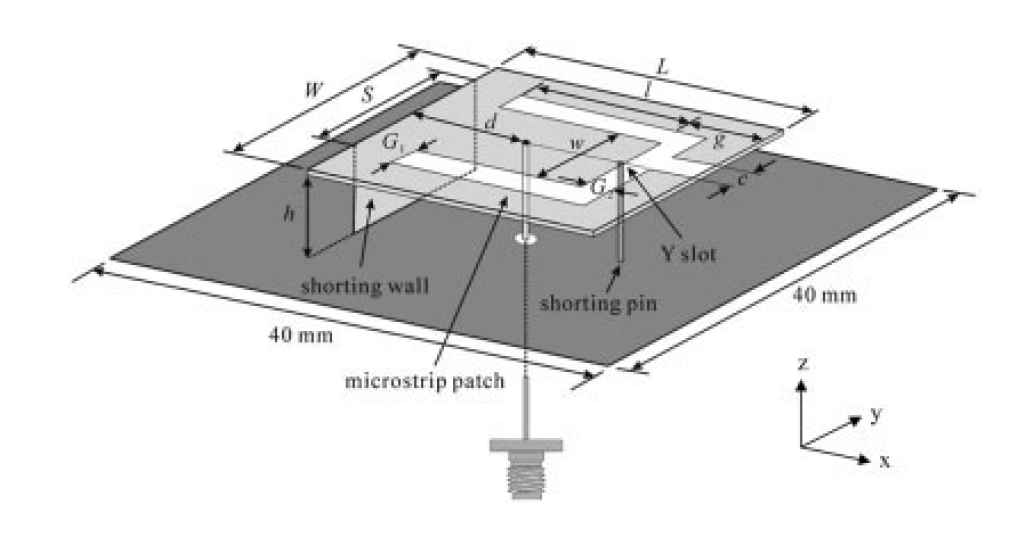
\includegraphics[height=5cm]{figs/30.png}
		\end{figure}
\end{frame}

\begin{frame}{研究现状——{\normalsize 应用于WLAN的双频天线研究现状}}
	\qquad 一种应用于WLAN 频段的半圆形开槽双频定向PIFA
	天线,该天线完全覆盖IEEE 802.11a/b/n/ac频段,
	且具有较低的剖面。 然而,相比于微带天线,PIFA
	天线方向图不圆度较差,且增益较低。		
	\begin{figure}[htbp]
				\centering
				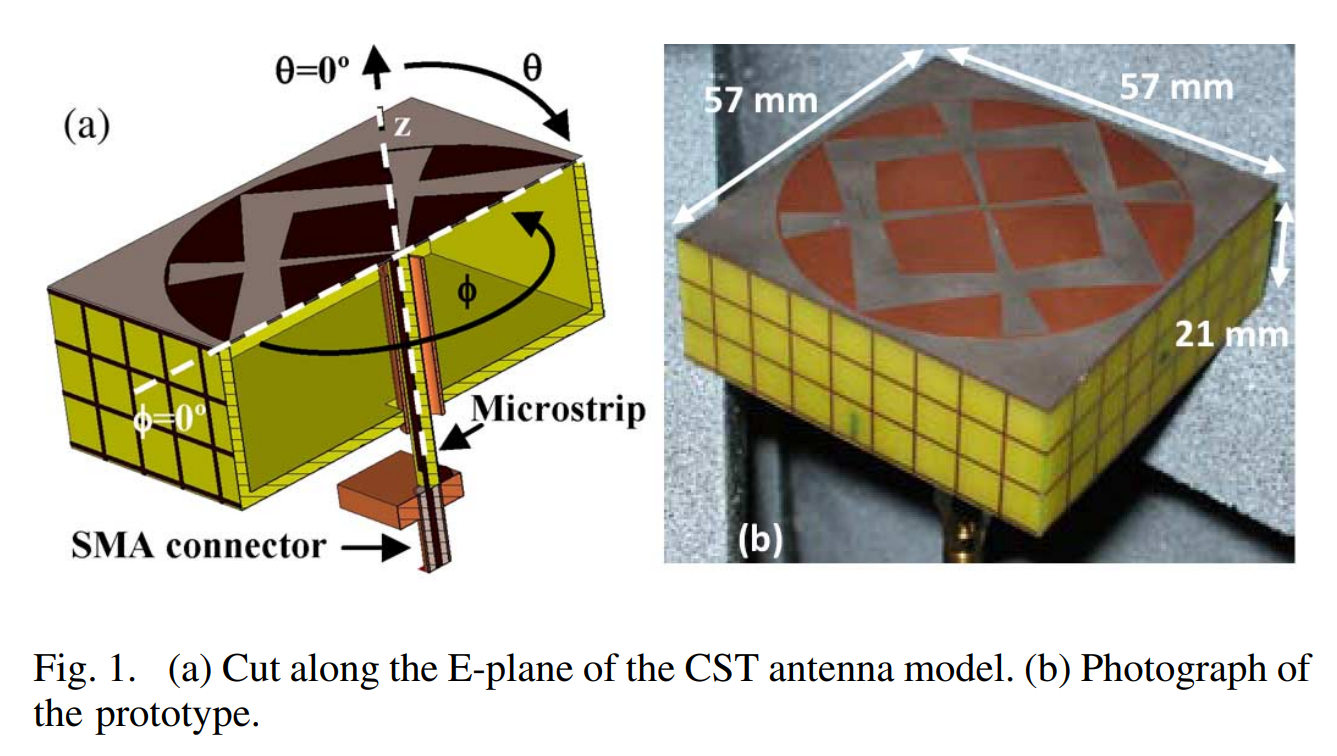
\includegraphics[height=5cm]{figs/29.png}
			\end{figure}
\end{frame}




\section{理论分析}
\begin{frame}{理论分析}
\qquad 在上述研究的基础上,本研究提出一款应用于WLAN的低剖面微带天线,
	可以完全覆盖IEEE 802.11a/b/n/ac频段,具有较低的剖面,且增益
	较高。
\end{frame}

\begin{frame}{理论分析——{\normalsize 微带天线实现双频的方法}}
	\begin{itemize}
		\item 微带天线可用{\Large 电抗加载}的方法实现双频工作\pause
		\item 根据空腔模型理论,
		薄基片的微带天线在主模谐振频率附近的输入阻
		抗$Z_{in}$可等效为$Z_{in}=R+jX_{f1}+jX_{f2}$,
		其中$X_{f1}$为主模并联谐振等效电路的“谐振”电抗,
		$X_{f2}$为其他模的合成效应。\pause
		\item 当天线谐振时,$X_{f1}+X_{f2}=0$
	\end{itemize}
	
\end{frame}
\begin{frame}{理论分析——{\normalsize 微带天线实现双频的方法}}
	\begin{itemize}
		\item 若用一个电抗对微带天线进行加载,则上述的特征方程为
		$X_{f1}+X_{f2}+X_{l}=0$,调节$X_l$的值,可以获得两个零点,这便是
		电抗加载方法的基本原理。其中,对于缝隙加载而言,$X_l$是缝隙参数
		(包括长度、宽度、位置等)的函数,因此可以调整这些参数来改变两个谐振频率的距离。
		\end{itemize}
\end{frame}


\begin{frame}{理论分析——{\normalsize 微带天线实现双频的方法}}
	\begin{itemize}
		\item 加载的缝隙形状可以有很多种,比较
		实用的有一种在天线贴片中间位置加载一个两
		臂很短的U形缝隙。加载的U形槽分割了矩形贴
		片上的电流分布,使贴片表现出双频效应:馈电
		点到天线贴片两个辐射边的电流路径由于缝隙的
		存在被拉长,降低了天线贴片的谐振频率,从而
		使贴片整体尺寸小于半波长;所以可以通过改变
		贴片的长度来调整低频段的中心谐振频率。
	\end{itemize}
\end{frame}
\begin{frame}{理论分析——{\normalsize 微带天线实现双频的方法}}
	\begin{itemize}
		\item 而又由于U形缝隙的底边对电流
		的影响形成了一个较高的谐振频率;由于
		从馈电点到贴片边缘的电流被缝隙阻挡,
		则由这个U形缝隙所围区域产生一个假想的
		辐射贴片,所以可以通过改变缝隙的长度来
		改变高频段的中心谐振频率。其中,U形缝隙
		的两臂因为是顺着电流方向,所以对频率的影响
		不是很大,但是这样的对称结构可以获得较好
		的极化特性,也对阻抗匹配起到调节作用。
		\end{itemize}
\end{frame}

\begin{frame}{理论分析——{\normalsize 微带天线实现双频的方法}}
	\begin{itemize}
		\item 本课题所使用的天线基于加载了U形
		缝隙的贴片天线进行改进。天线贴片由矩形
		内外贴片组成,用U型缝隙将其隔开,同时使
		用三个矩形电桥进行链接,并且在外贴片上
		还加载了一根短路探针,该探针相当于在天
		线的等效电路中引入了一个等效电感,从而形
		成一个并联谐振电路,对天线的低频谐振频率
		起到了调谐的作用。
	\end{itemize}
\end{frame}

\section{天线结构与设计}
\begin{frame}{天线结构与设计——{\normalsize 天线组成}}
	\qquad 天线结构如下图所示,{\large  \bfseries 由
	{空气层},上下两层FR4介质及其印刷导体组成
	。天线的辐射单元由印刷在
	上层介质基板上的U
型外贴片、矩形内贴片以及它们之间的矩形连接桥组成。}U 型外
贴片外围总尺寸为$L_2 \times W_2$
;矩形内贴片的尺寸为$L_4 \times W_4$
;矩形连
接桥A 的长度为$W_a$
,矩形连接桥B 和C 的长度都为$W_b$。该天线
采用同轴探针馈电,馈电点在距中心点O 的距离为$x_f$
的$x$ 轴上。
加载的短路探针D 在U 型外贴片处与微带天线接地面短接。
\end{frame}
\begin{frame}{天线结构与设计}
	\begin{figure}[htbp]
		\centering
		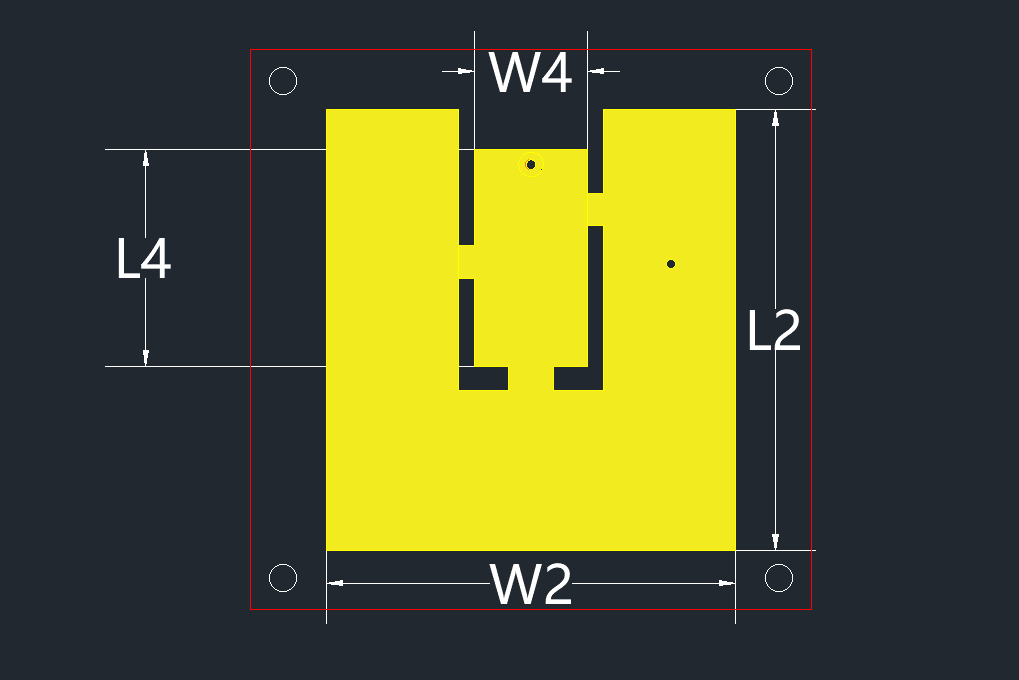
\includegraphics[width=8cm]{figs/f3.png}
		\caption{天线结构图(正面)}
	\end{figure}
\end{frame}
\begin{frame}{天线结构与设计}
	\begin{figure}[htbp]
		\centering
		
\includegraphics[width=6cm]{figs/f4.png}
		\caption{天线结构图(背面)}
	\end{figure}
\end{frame}



\begin{frame}{天线结构与设计}
	\qquad 天线的最初设计源于天线I,如图(\ref{ff16})所示。
	天线辐射贴片可以看作是矩形贴片加载
	一个U 型槽形成。 
	\begin{figure}[htbp]
		\centering
		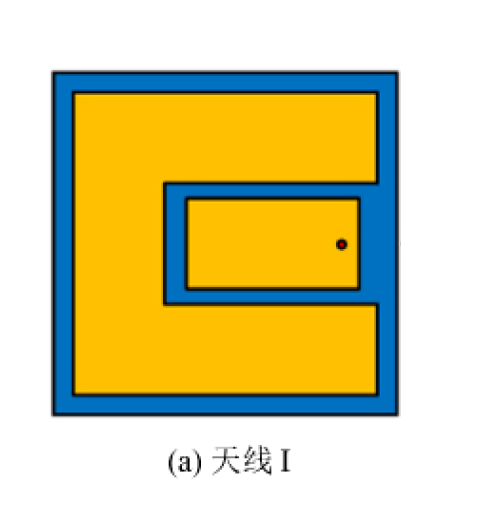
\includegraphics[width=3.5cm]{figs/16.png}
		\caption{天线的设计过程}
		\label{ff16}
	\end{figure}
	 
	
\end{frame}
\begin{frame}{天线结构与设计}
\qquad 天线II在U 型外贴片和矩形内贴片之间的
	槽中增加了三个矩形连接桥A、B 和C.

	\begin{figure}[htbp]
		\centering
		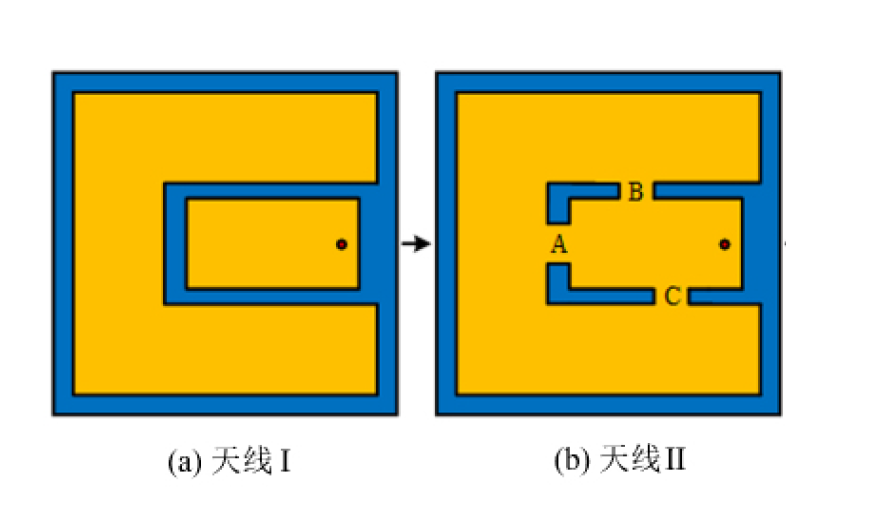
\includegraphics[width=7cm]{figs/17.png}
		\caption{天线的设计过程}
		\label{3}
	\end{figure}
\end{frame}


\begin{frame}{天线结构与设计}
	\qquad 在天线II 的基础上,天线
	III 在U 型外贴片上加载了一根短路探针D。
		\begin{figure}[htbp]
			\centering
			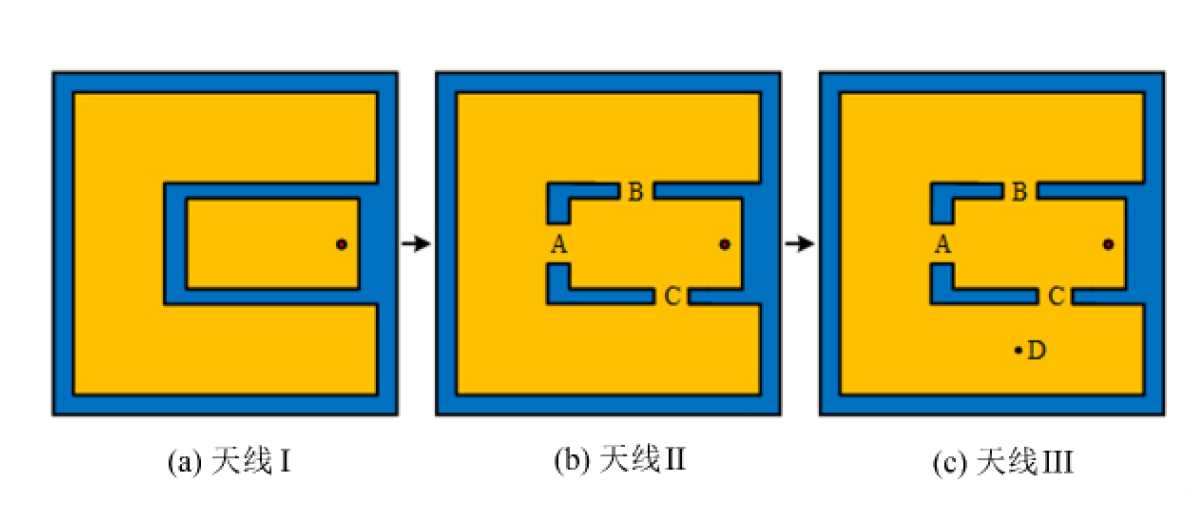
\includegraphics[width=10cm]{figs/3.png}
			\caption{天线的设计过程}
			\label{3}
		\end{figure}
		
	\end{frame}

\begin{frame}{天线结构与设计——{\normalsize 天线等效电路图}}

	\qquad 这相当于在天线的等效电路中引入了一个等效电感L3
	,从而形成了一个并联谐振电路,该短路探针等效
	电感对天线的低频谐振频率起到调谐的作用。
	\begin{figure}[htbp]
		\centering
		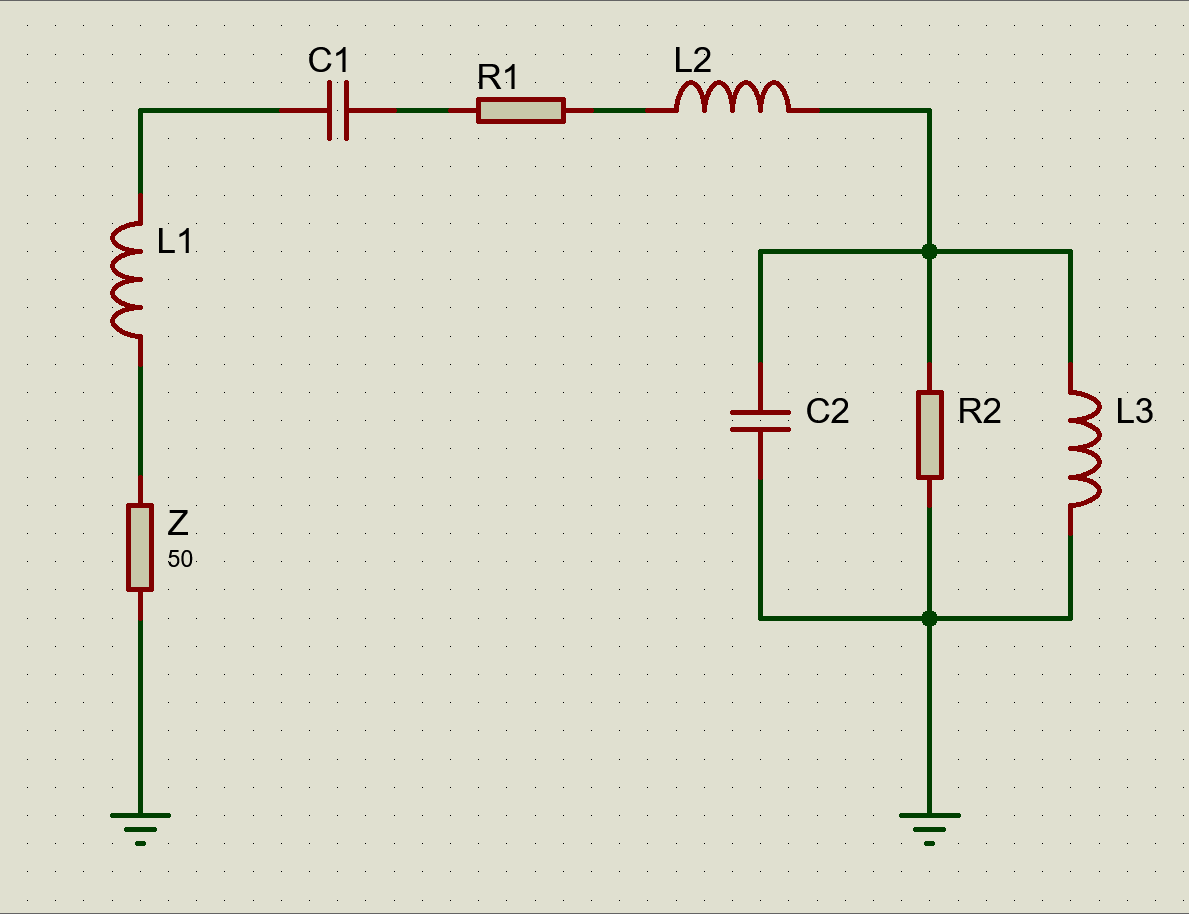
\includegraphics[width=5cm]{figs/f2.png}
		\caption{天线等效电路图 }
	\end{figure}
\end{frame}


\begin{frame}{天线结构与设计——{\normalsize 天线等效电路图}}
	\qquad 探针阻抗设为R2
	,如图(\ref{f222})所示. 从图(\ref{f222})中可以看出,整个天
	线可以等效为串联谐振电路和并联谐振电路的组合,
	并激励出了两个相邻的谐振模式,天线的频带宽度
	由此得到了展宽。
	\begin{figure}[htbp]
		\centering
		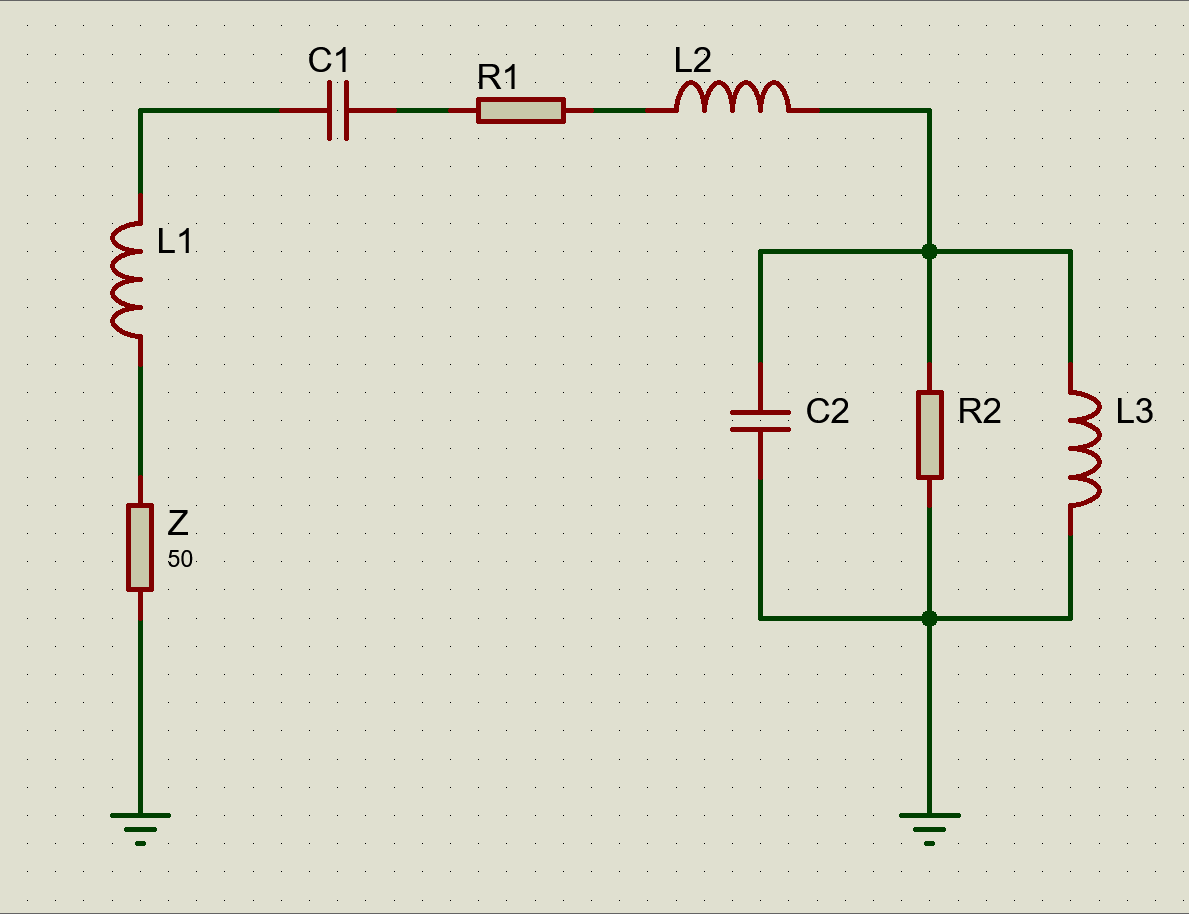
\includegraphics[width=5cm]{figs/f2.png}
		\caption{天线等效电路图 }
		\label{f222}
	\end{figure}
\end{frame}


\section{建模仿真}
\begin{frame}{建模仿真}
	\qquad 在建模前要明确天
线的尺寸,并计算出同轴馈电线的尺寸和材料,
以产生进行阻抗匹配。\pause

\qquad 根据同轴电缆特征阻抗为$50\Omega$,选取同轴线填充材料
为$Teflon$,其相对介电常数为2.1,根据同轴电缆特征阻抗计算公式:
\begin{theorem}
$$Z_0=\frac{60}{\sqrt{\varepsilon_r}}\times\ln\frac{D}{d}
$$
\end{theorem}
取同轴线半径为4.6mm,同轴线内导体半径为1.36mm。
\end{frame}
\subsection*{HFSS模型}
\begin{frame}{建模仿真——{\normalsize HFSS模型}}
	\begin{figure}[htbp]
		\centering
		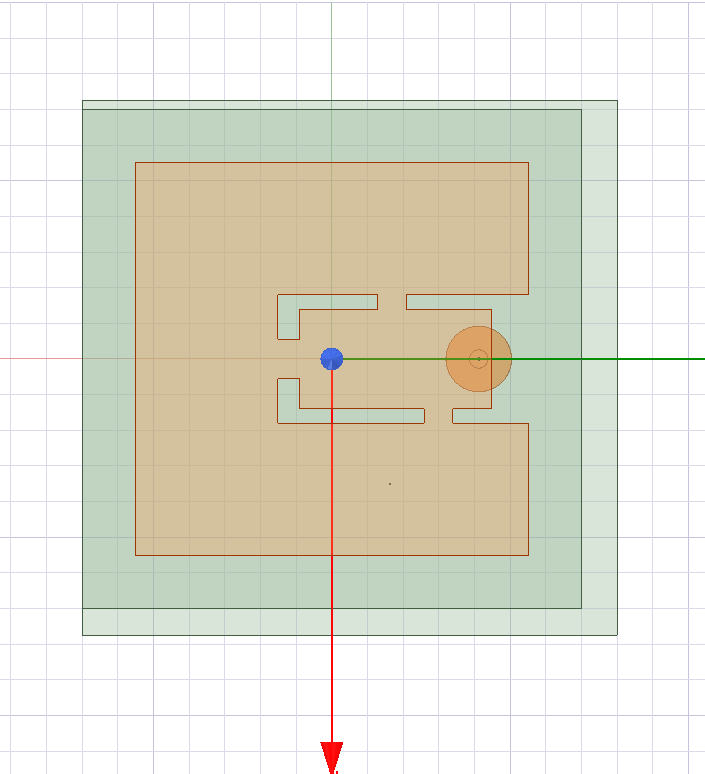
\includegraphics[width=5cm]{figs/4.png}
		\caption{微带天线HFSS模型}
		\label{f2}
	\end{figure}
\end{frame}

\begin{frame}{建模仿真——{\normalsize HFSS模型}}
	\begin{figure}[htbp]
		\centering
		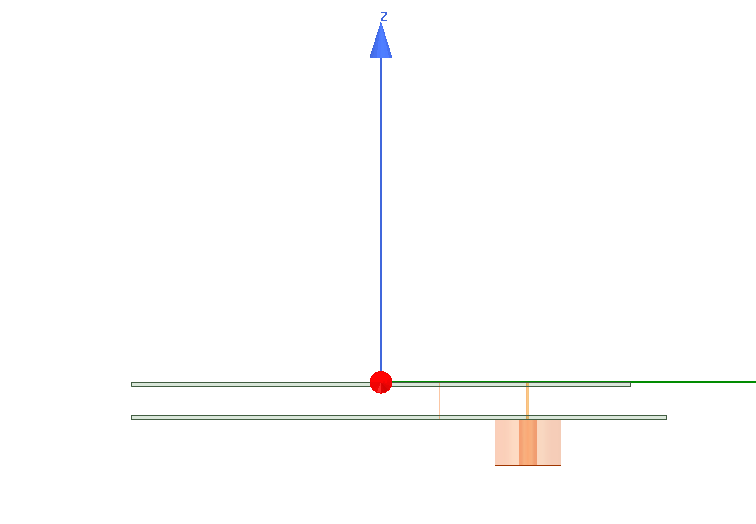
\includegraphics[width=7cm]{figs/5.png}
		\caption{微带天线HFSS模型}
		\label{f2}
	\end{figure}
\end{frame}

\begin{frame}{建模仿真——{\normalsize HFSS模型}}
	\begin{figure}[htbp]
		\centering
		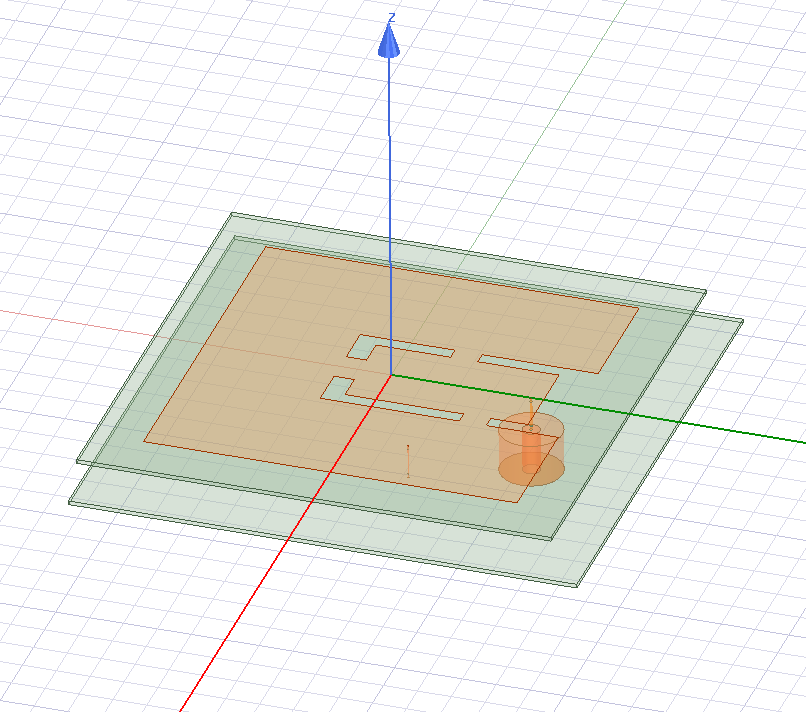
\includegraphics[width=6cm]{figs/6.png}
		\caption{微带天线HFSS模型}
		\label{f2}
	\end{figure}
\end{frame}

\begin{frame}{建模仿真——{\normalsize HFSS模型}}
	\begin{figure}[htbp]
		\centering
		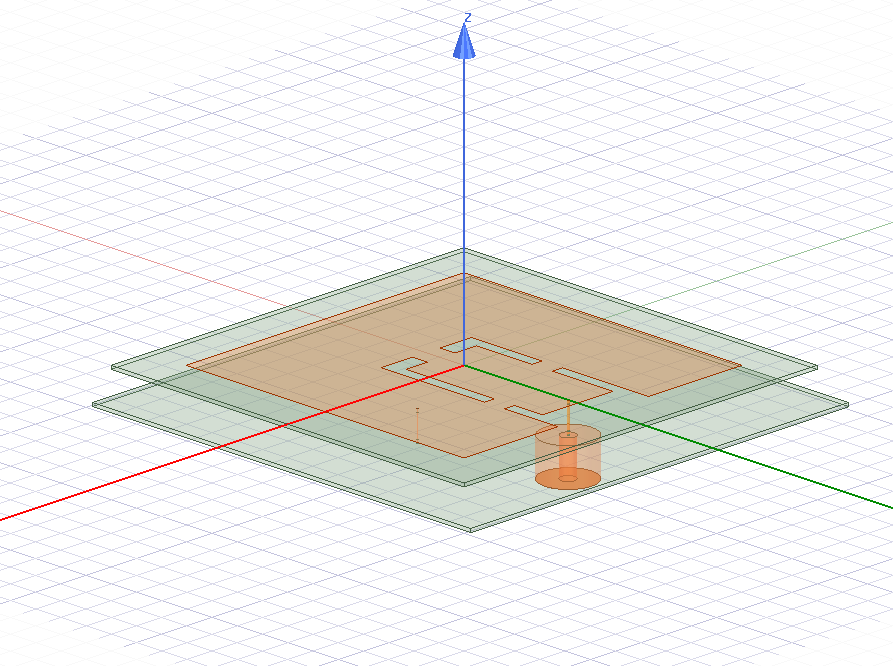
\includegraphics[width=6cm]{figs/13.png}
		\caption{微带天线HFSS模型}
		\label{f2}
	\end{figure}
\end{frame}
\subsection*{HFSS仿真}
\begin{frame}{建模仿真}
\qquad 建立模型之后设置1GHz-7GHz的扫频进行仿真。
仿真过程中发现:
\begin{enumerate}
	
	\item 短路点位置
	\item 短路导线尺寸
	\item 馈电点的位置 
	\item 馈电探针尺寸
\end{enumerate}
均对天线性能有影响,因此分别对这几个参数进行扫参。
	
\end{frame}

\begin{frame}{建模仿真——{\normalsize 短路点$y_d$坐标扫描}}
	\qquad 在保持短路导线的半径=0.5mm,
	馈电点位置$ x_f=20.6mm $,馈电探针半
	径0.6mm,短路点x坐标=8.2mm不变
	时,改变短路点的y坐标,其仿真结果如下图所示:
	\begin{figure}[htbp]
		\centering
		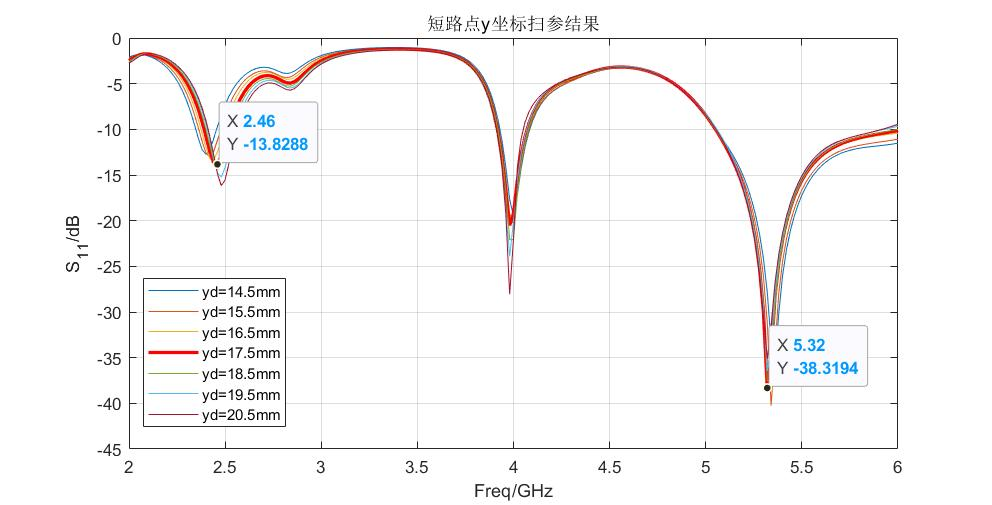
\includegraphics[height=5cm]{figs/20.jpg}
		%\caption{微带天线HFSS模型}
	\end{figure}	
\end{frame}

\begin{frame}{建模仿真——{\normalsize 短路点$y_d$坐标扫描}}
	\qquad 由扫参结果可以看出,当$ y_d=17.5mm $的时候,
	低频段的谐振点频率为2.45GHz,在2.4GHz和2.5GHz时的$S_{11}$分别为-10.74dB和-11.36dB,满足条件。
	而且随着$y_d$坐标
	的增大,谐振点频率向右移。但是$y_d$坐标的改变对高频
	段的谐振点频率影响很小。
	\begin{figure}[htbp]
		\centering
		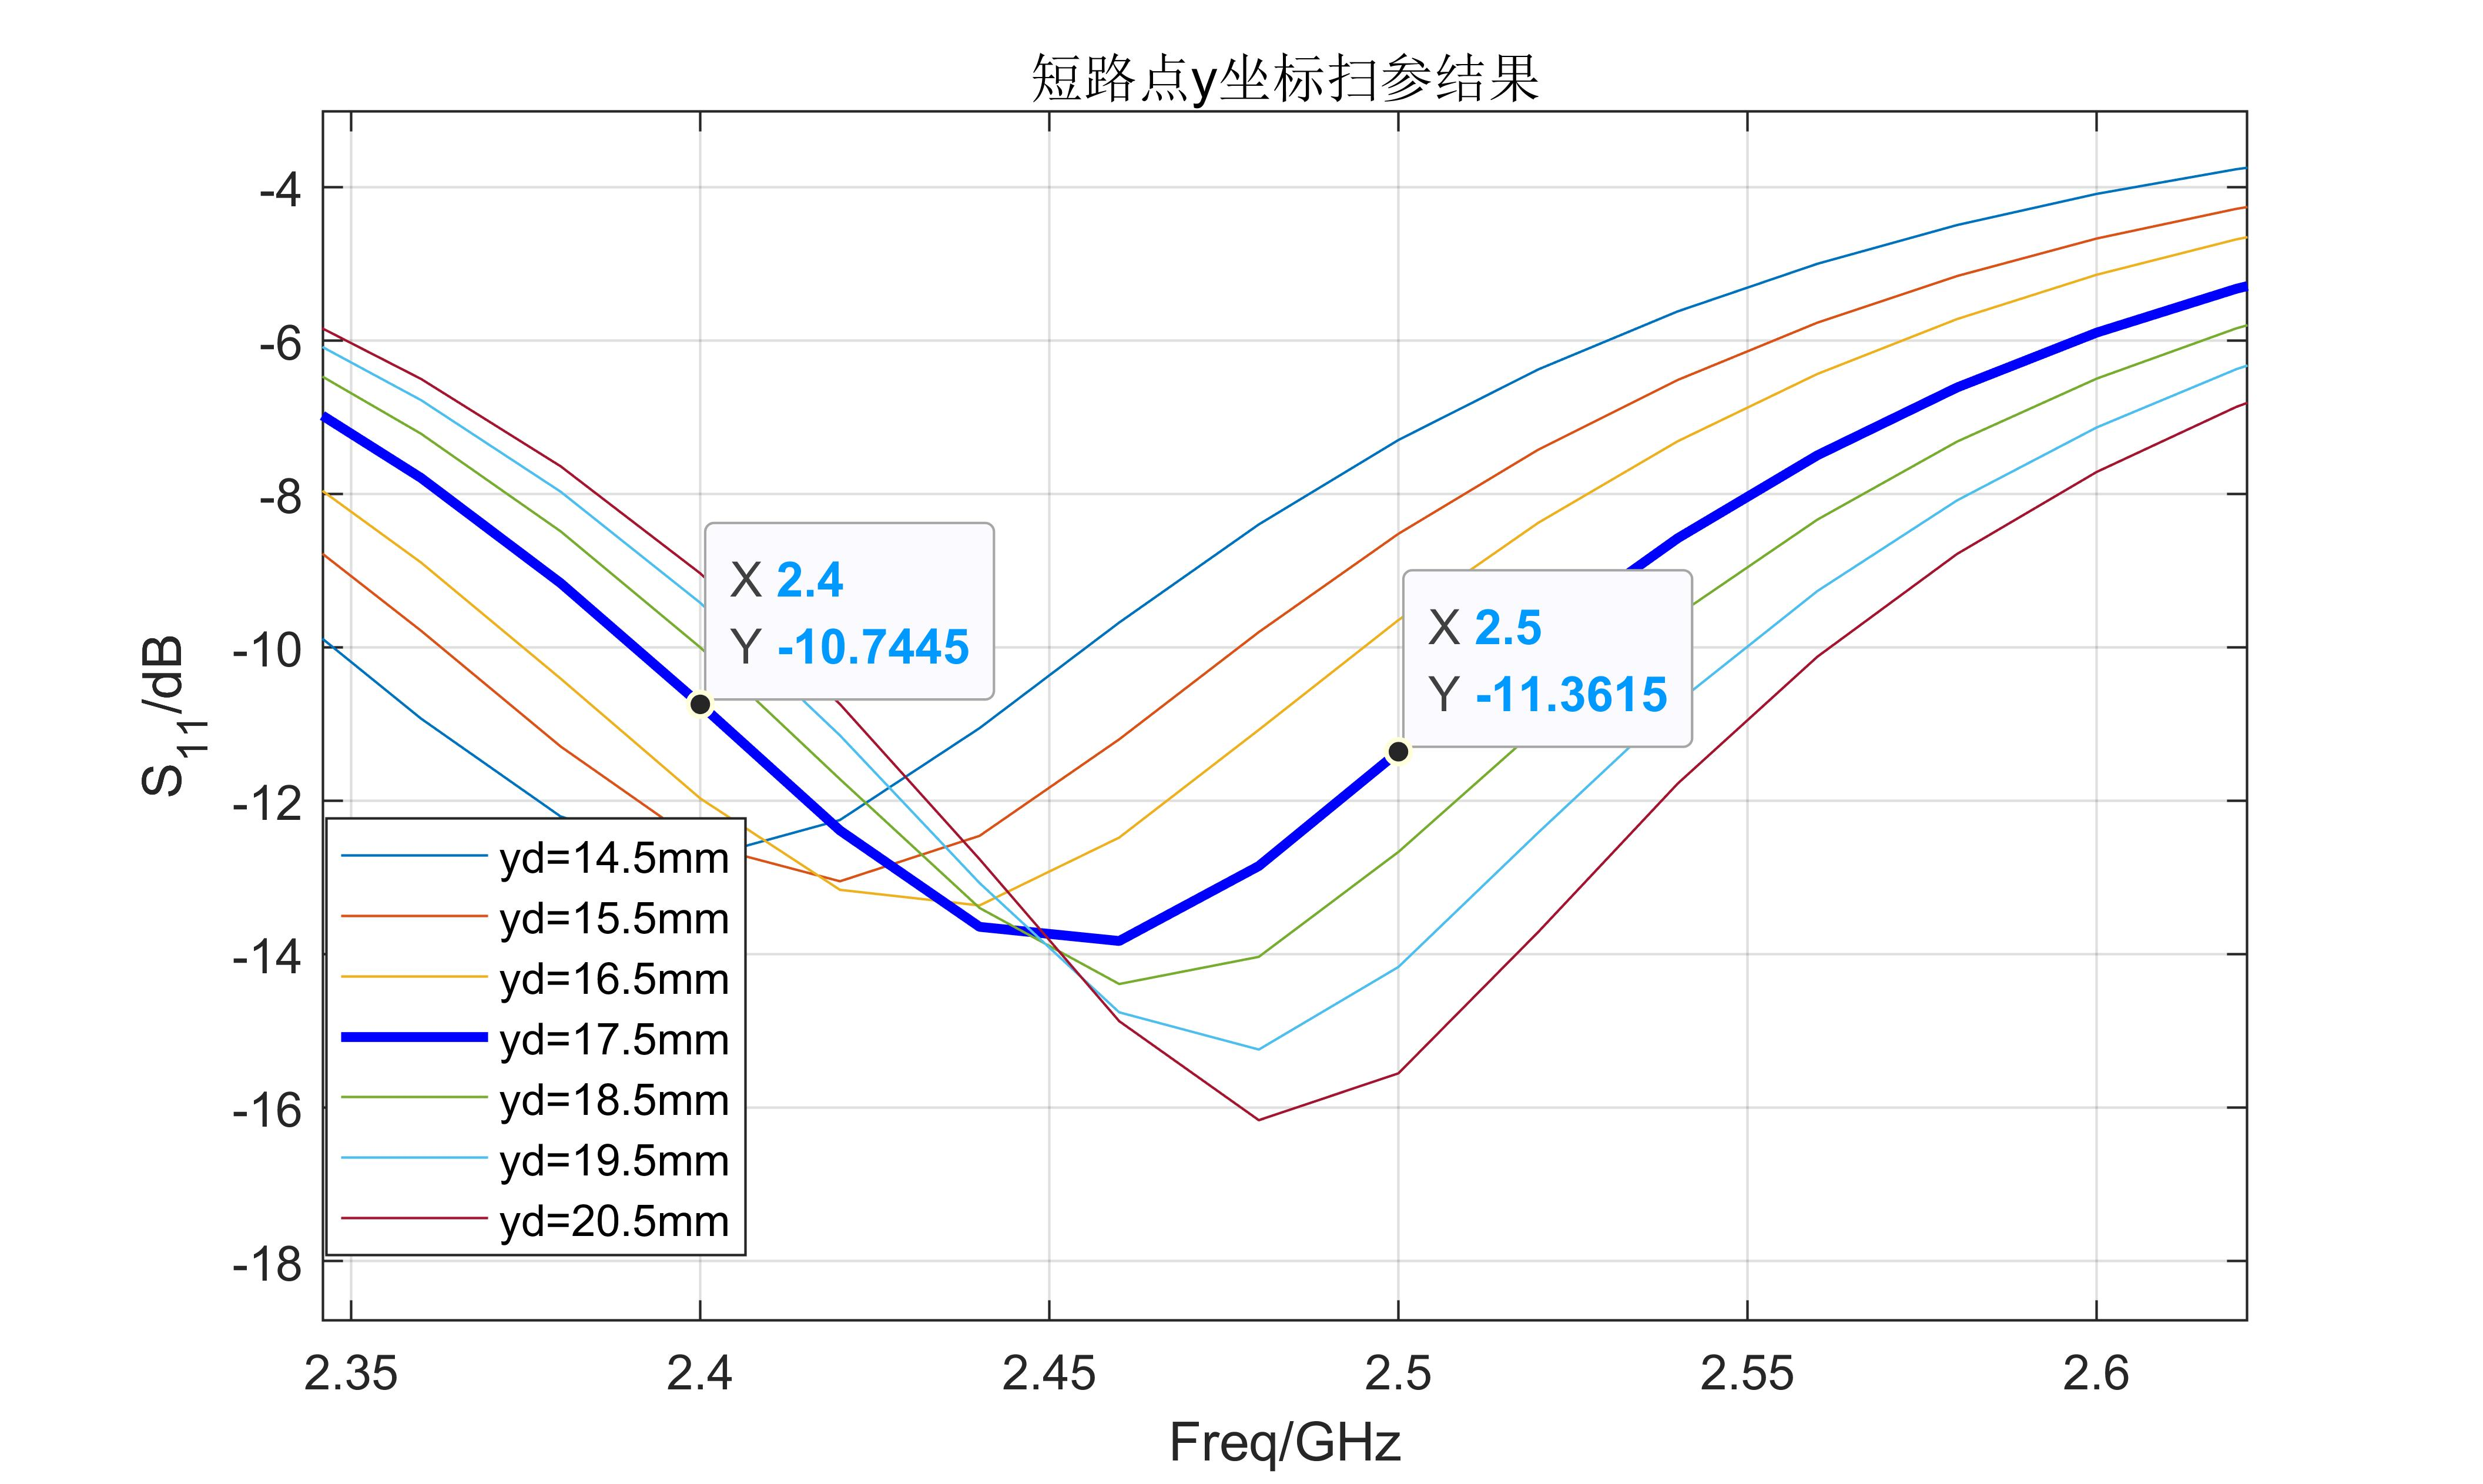
\includegraphics[height=4.5cm]{figs/21.jpg}
		%\caption{微带天线HFSS模型}
	\end{figure}	
\end{frame}


\begin{frame}{建模仿真——{\normalsize 短路导线半径的扫描}}
	\qquad 在保持馈电点位置$x_f=20.6mm$,
	馈电探针半径为0.6mm,
	短路点位置(8.2mm,17.5mm)不变时,
	改变短路导线的半径,其仿真结果如下图所示:
	\begin{figure}[htbp]
		\centering
		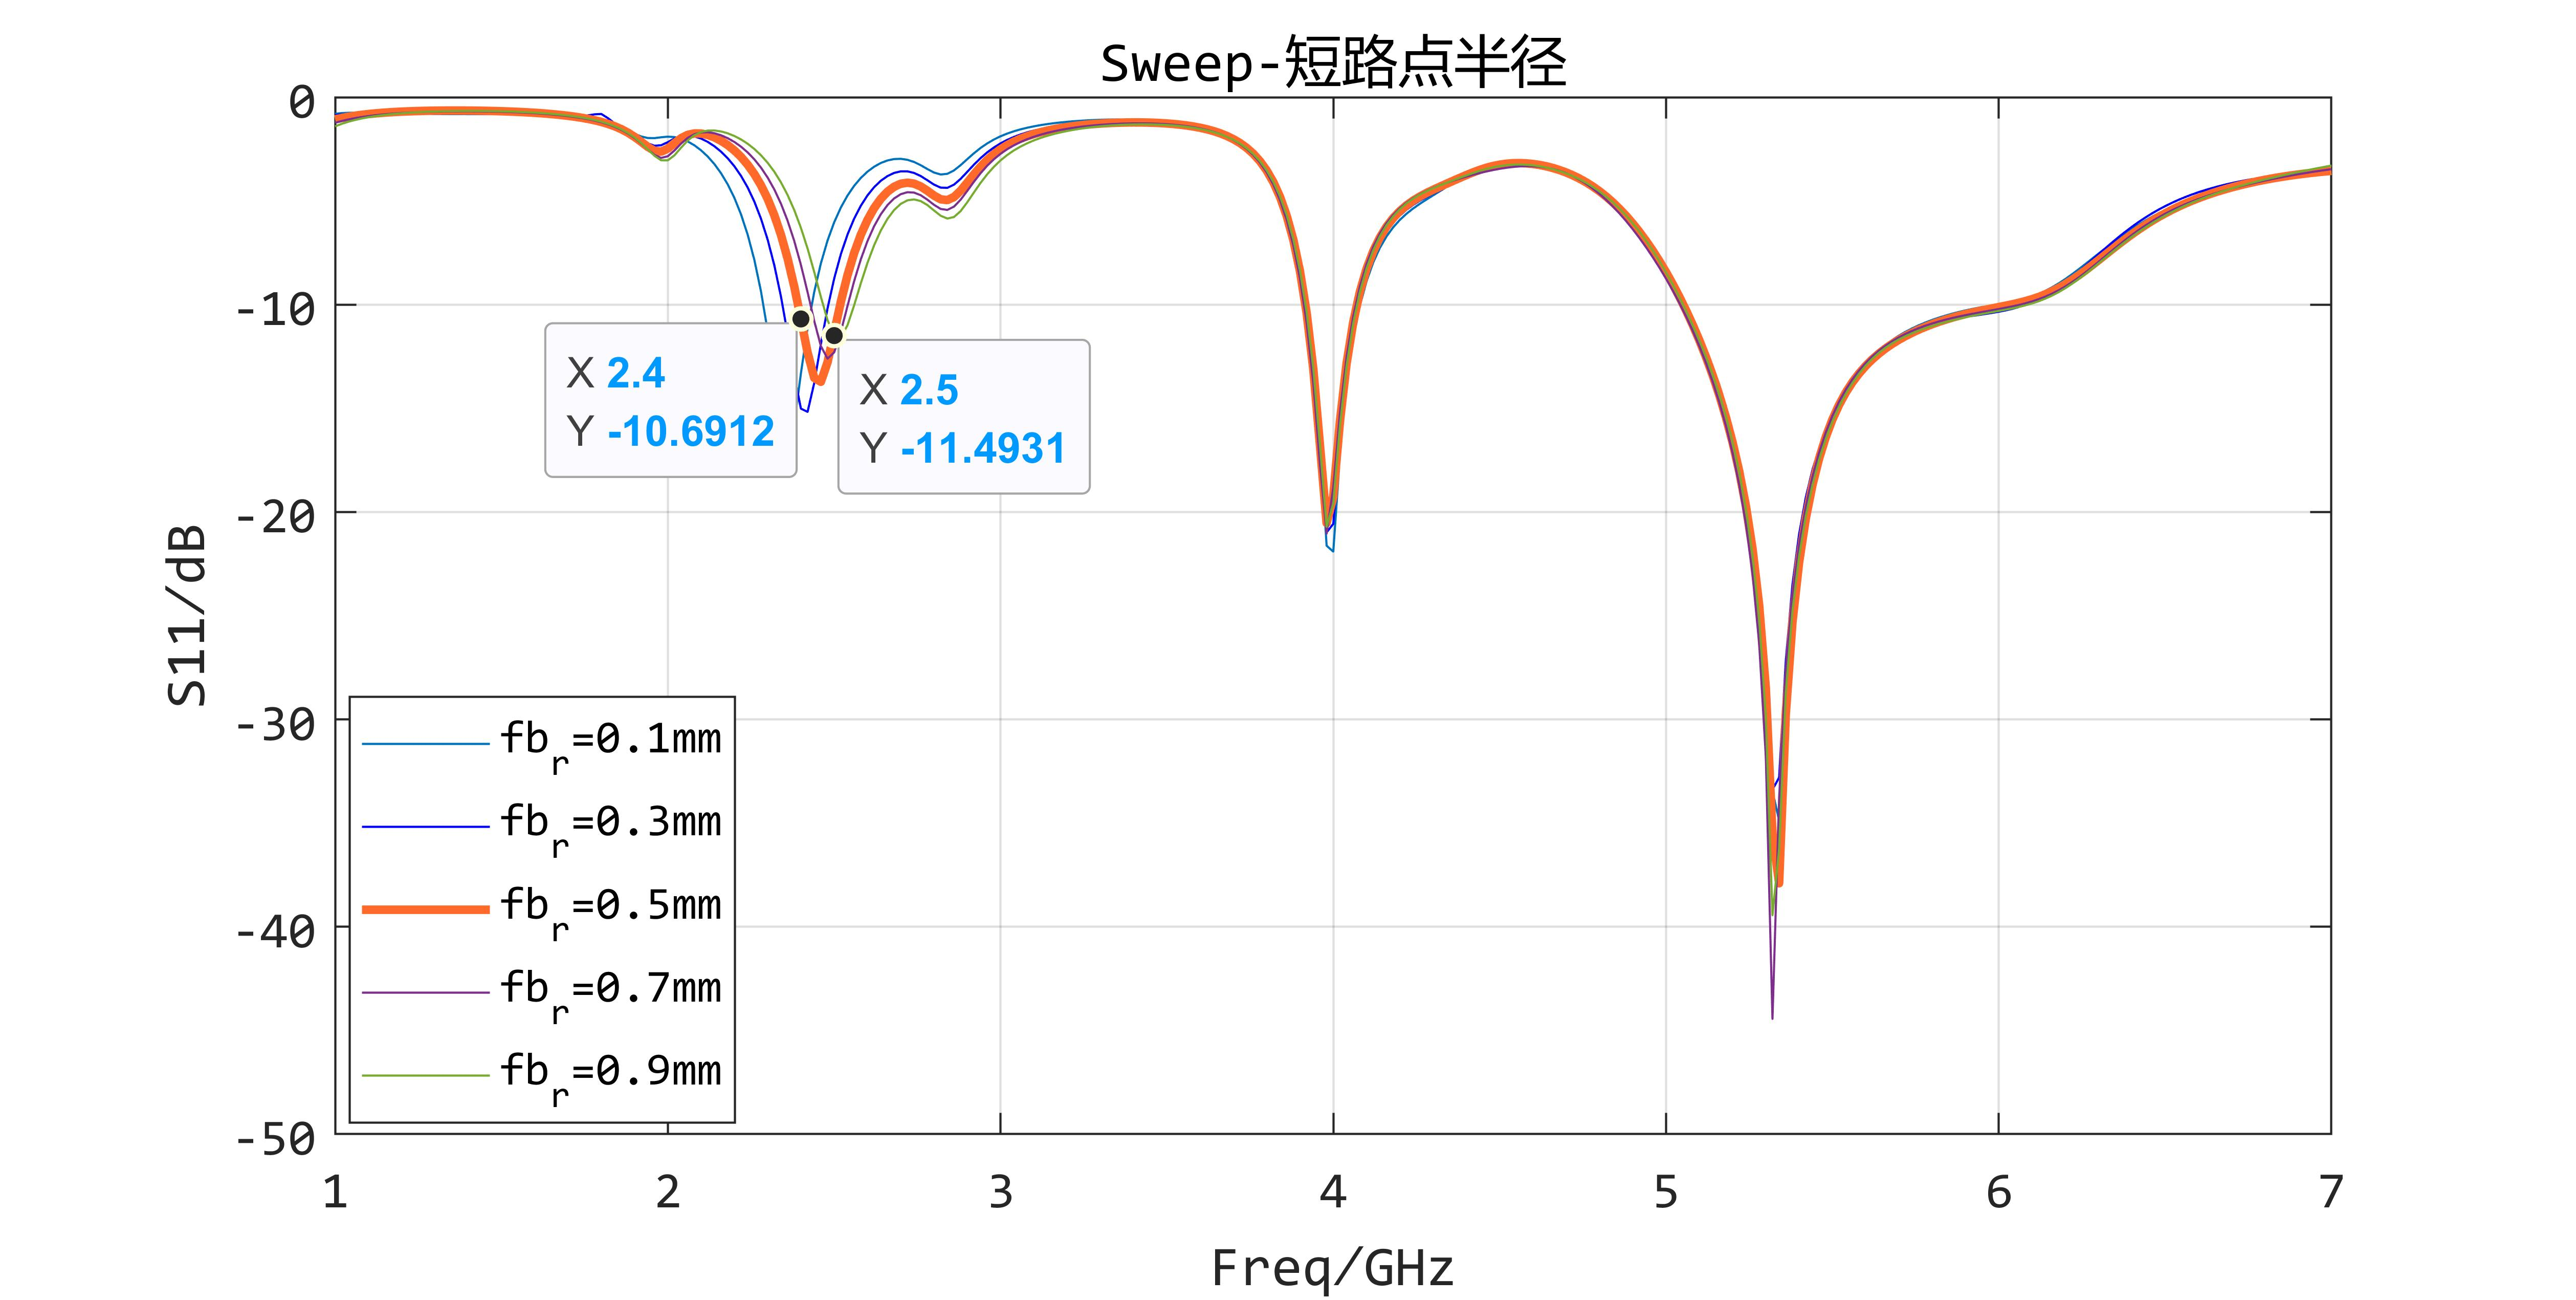
\includegraphics[height=5cm]{figs/short.jpg}
		%\caption{微带天线HFSS模型}
		\label{18}
	\end{figure}
\end{frame}
\begin{frame}{建模仿真——{\normalsize 短路导线半径的扫描}}
	\qquad 取短路导线半径为0.5mm时,此时2.4GHz和2.5GHz的$S_{11}$
	分别为-10.69dB和-11.49dB,满足条件,且最优,因此取短路导线半径
	为0.5mm。
	\begin{figure}[htbp]
		\centering
		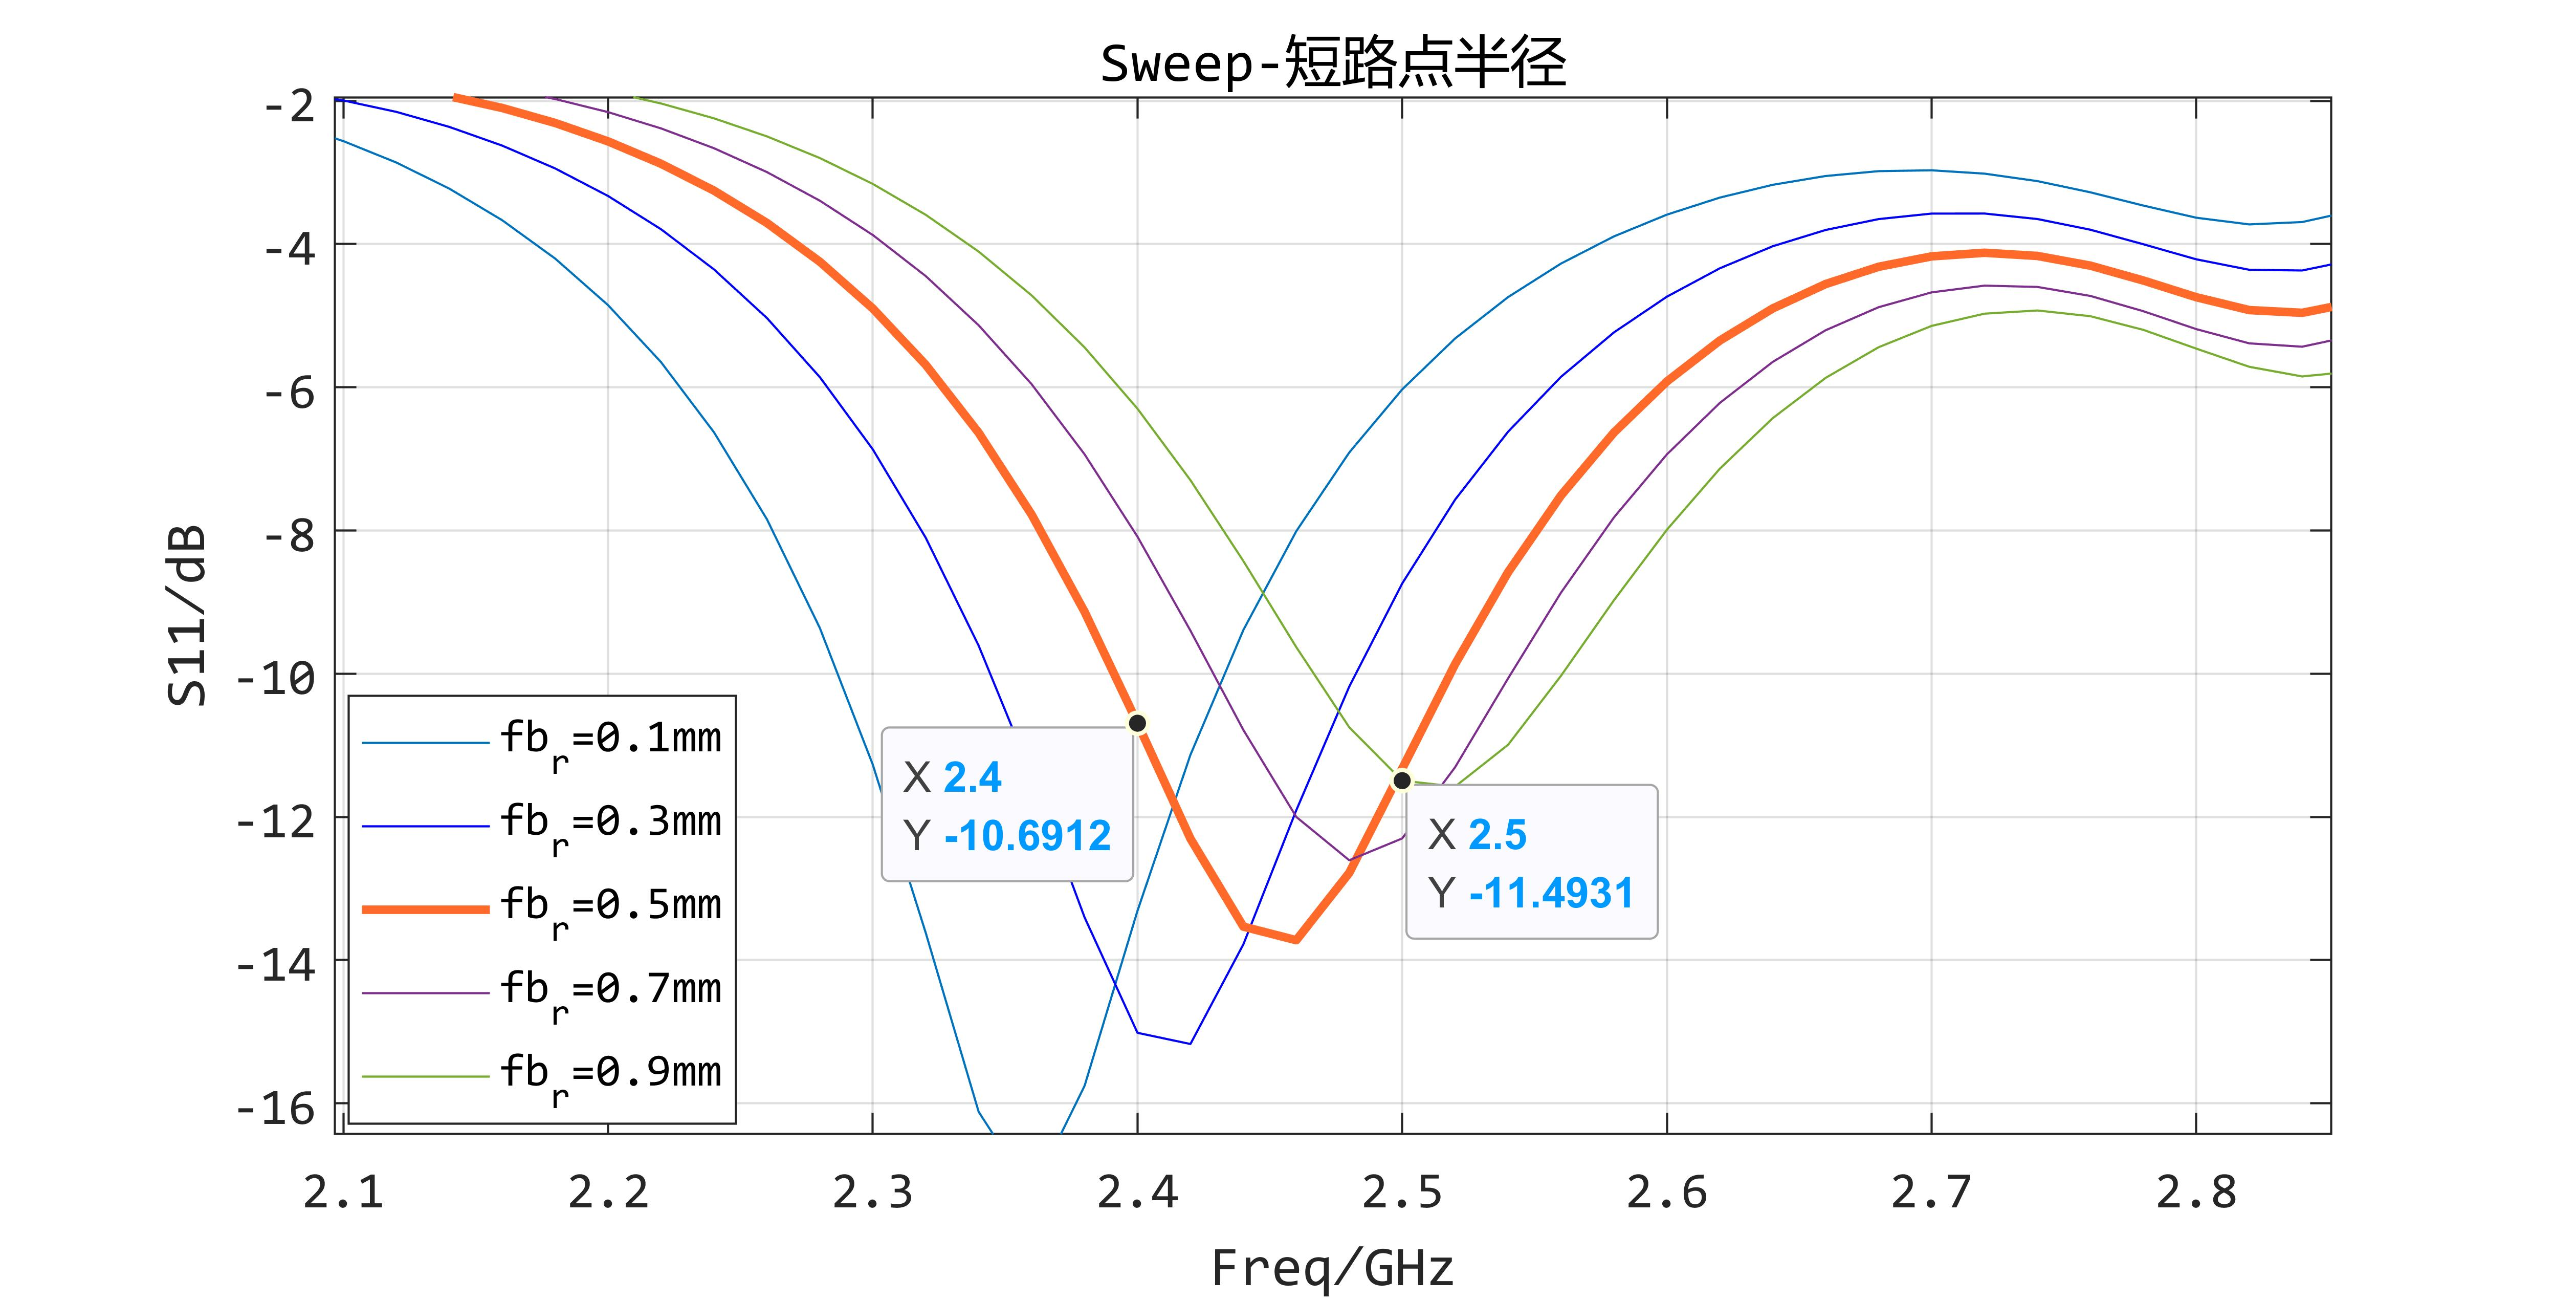
\includegraphics[height=5cm]{figs/short2.jpg}
		%\caption{微带天线HFSS模型}
		\label{18}
	\end{figure}
\end{frame}



\begin{frame}{建模仿真——{\normalsize 馈电点$x_f$坐标扫描}}
	\qquad 在保持短路导线的半径=0.5mm,
	馈电点位置$x_f=20.6mm$,馈电探针半
	径0.6mm,短路点$y$坐标=17.5mm不变时
	,改变馈电点的$x$坐标,其仿真结果如下图所示:
    \begin{figure}[htbp]
		\centering
		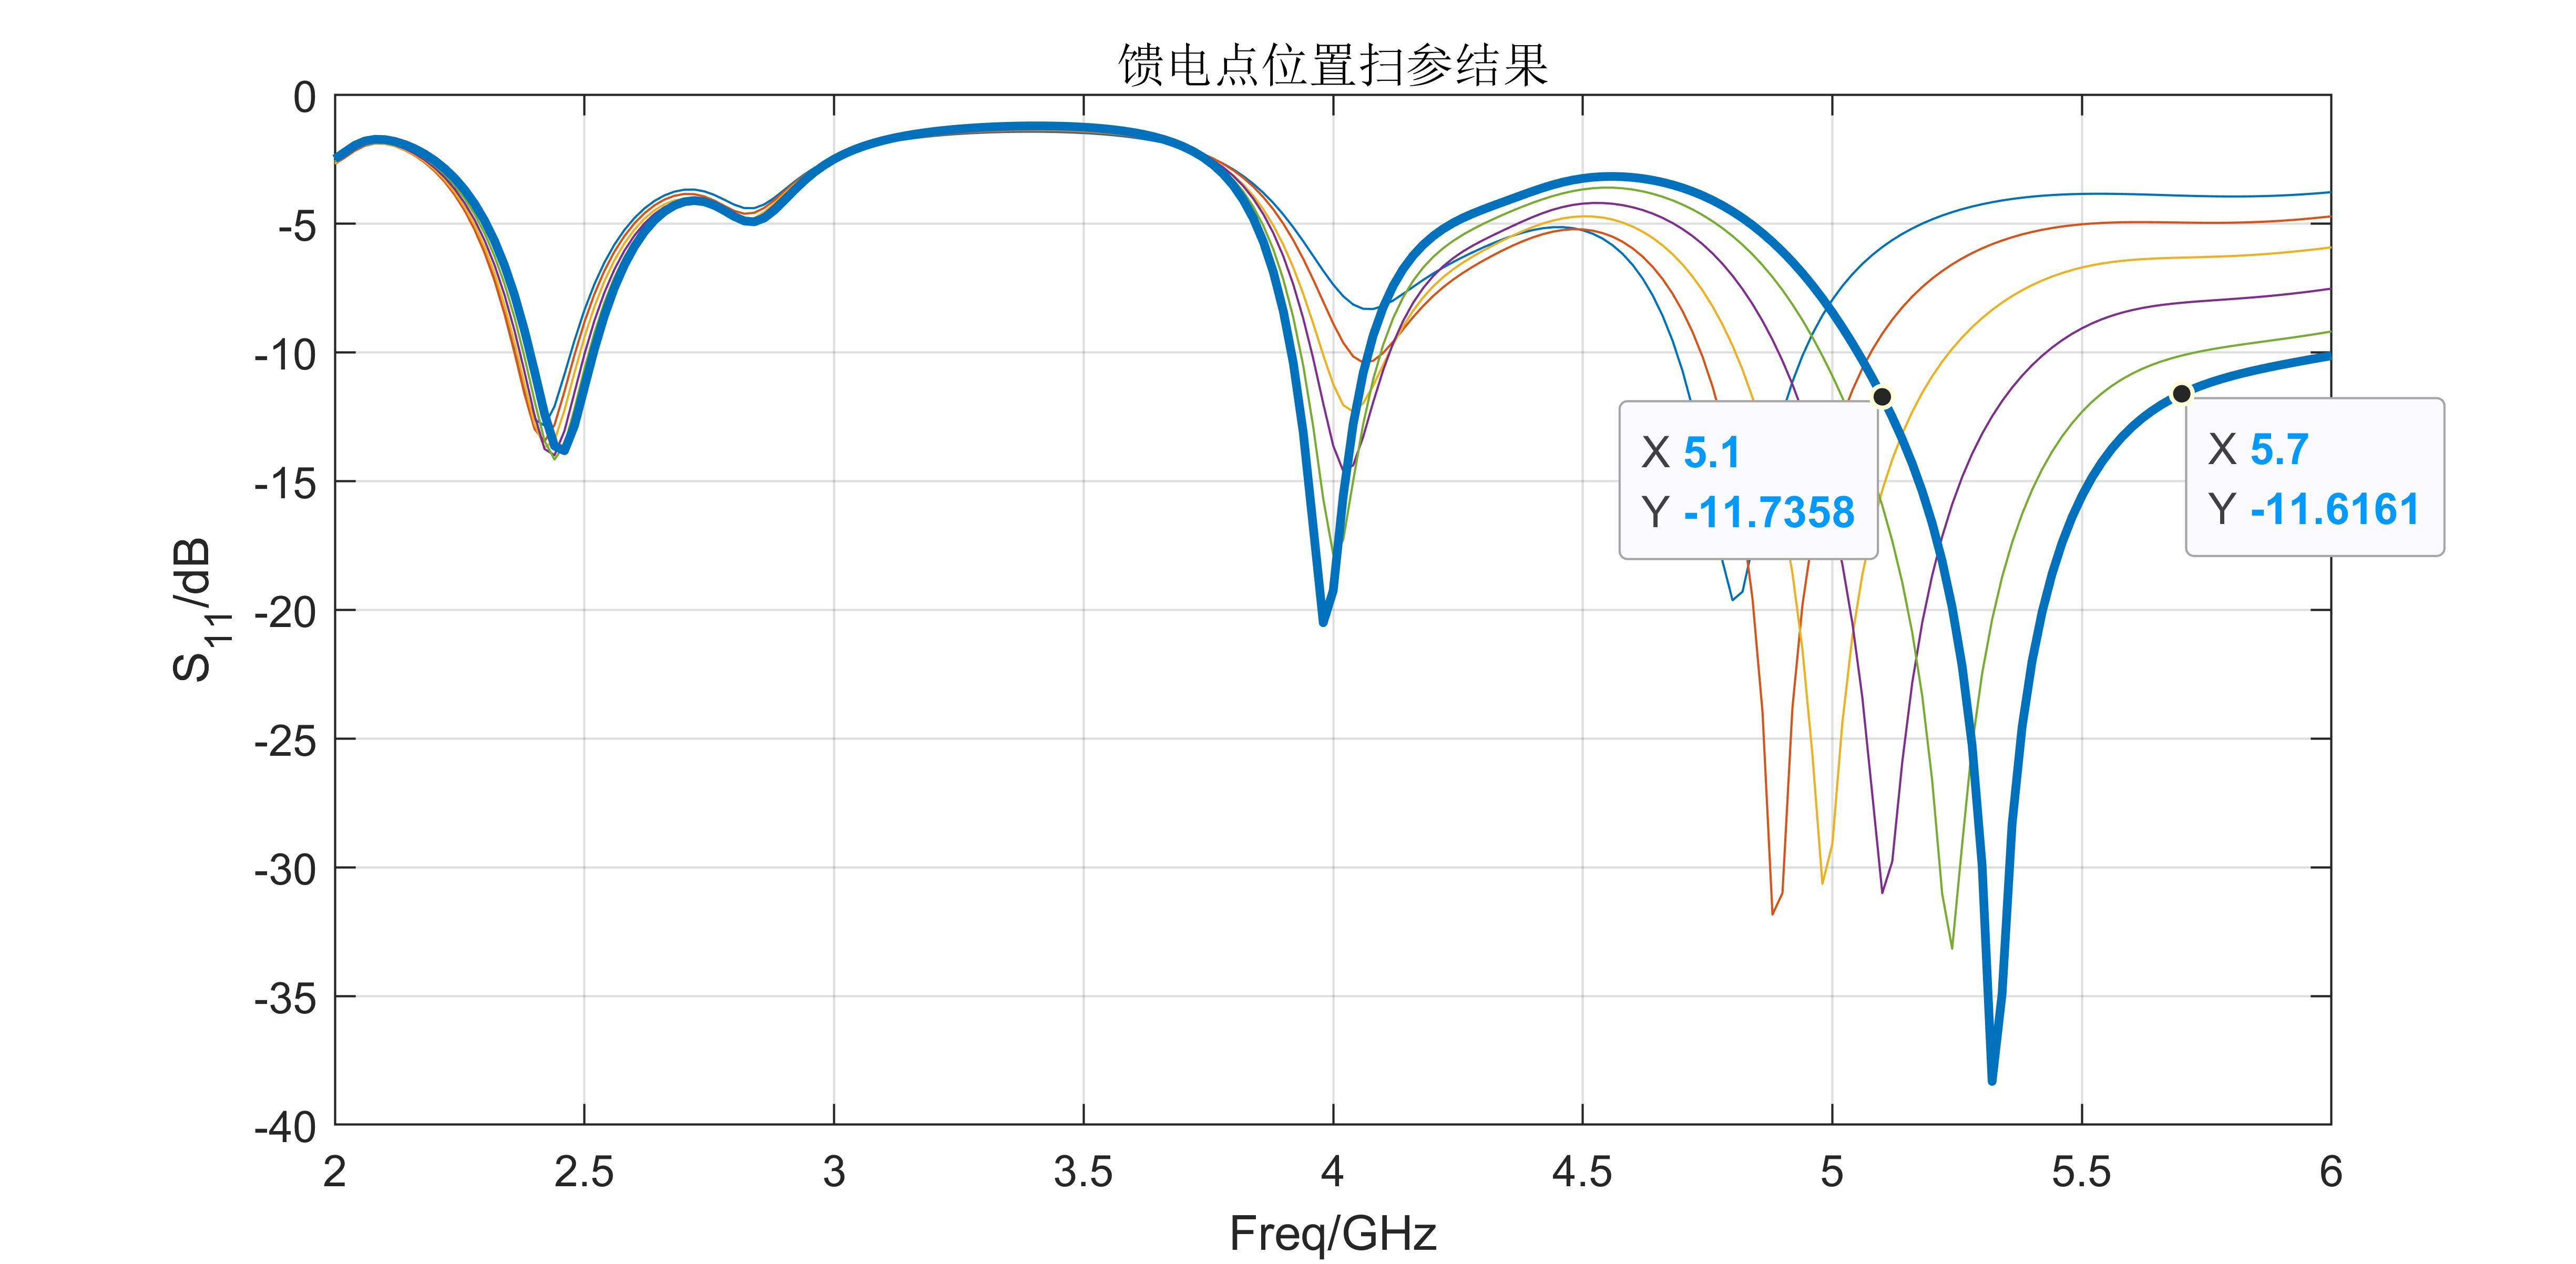
\includegraphics[height=5cm]{figs/feed_p1.jpg}
		%\caption{微带天线HFSS模型}
	\end{figure}
\end{frame}

\begin{frame}{建模仿真——{\normalsize 馈电点$x_f$坐标扫描}}
	\qquad 根据扫参的结果我们可
	以看出,馈电点位置主要影响高频
	段的谐振频率点,即随着$x_f$的增
	大,高频段的谐振频率点右移,
	可以看到,当$x_f=20.6mm$的时候,
	高频段谐振点频率与要求的5.5GHz频
	率最为接近。
	\begin{figure}[htbp]
		\centering
		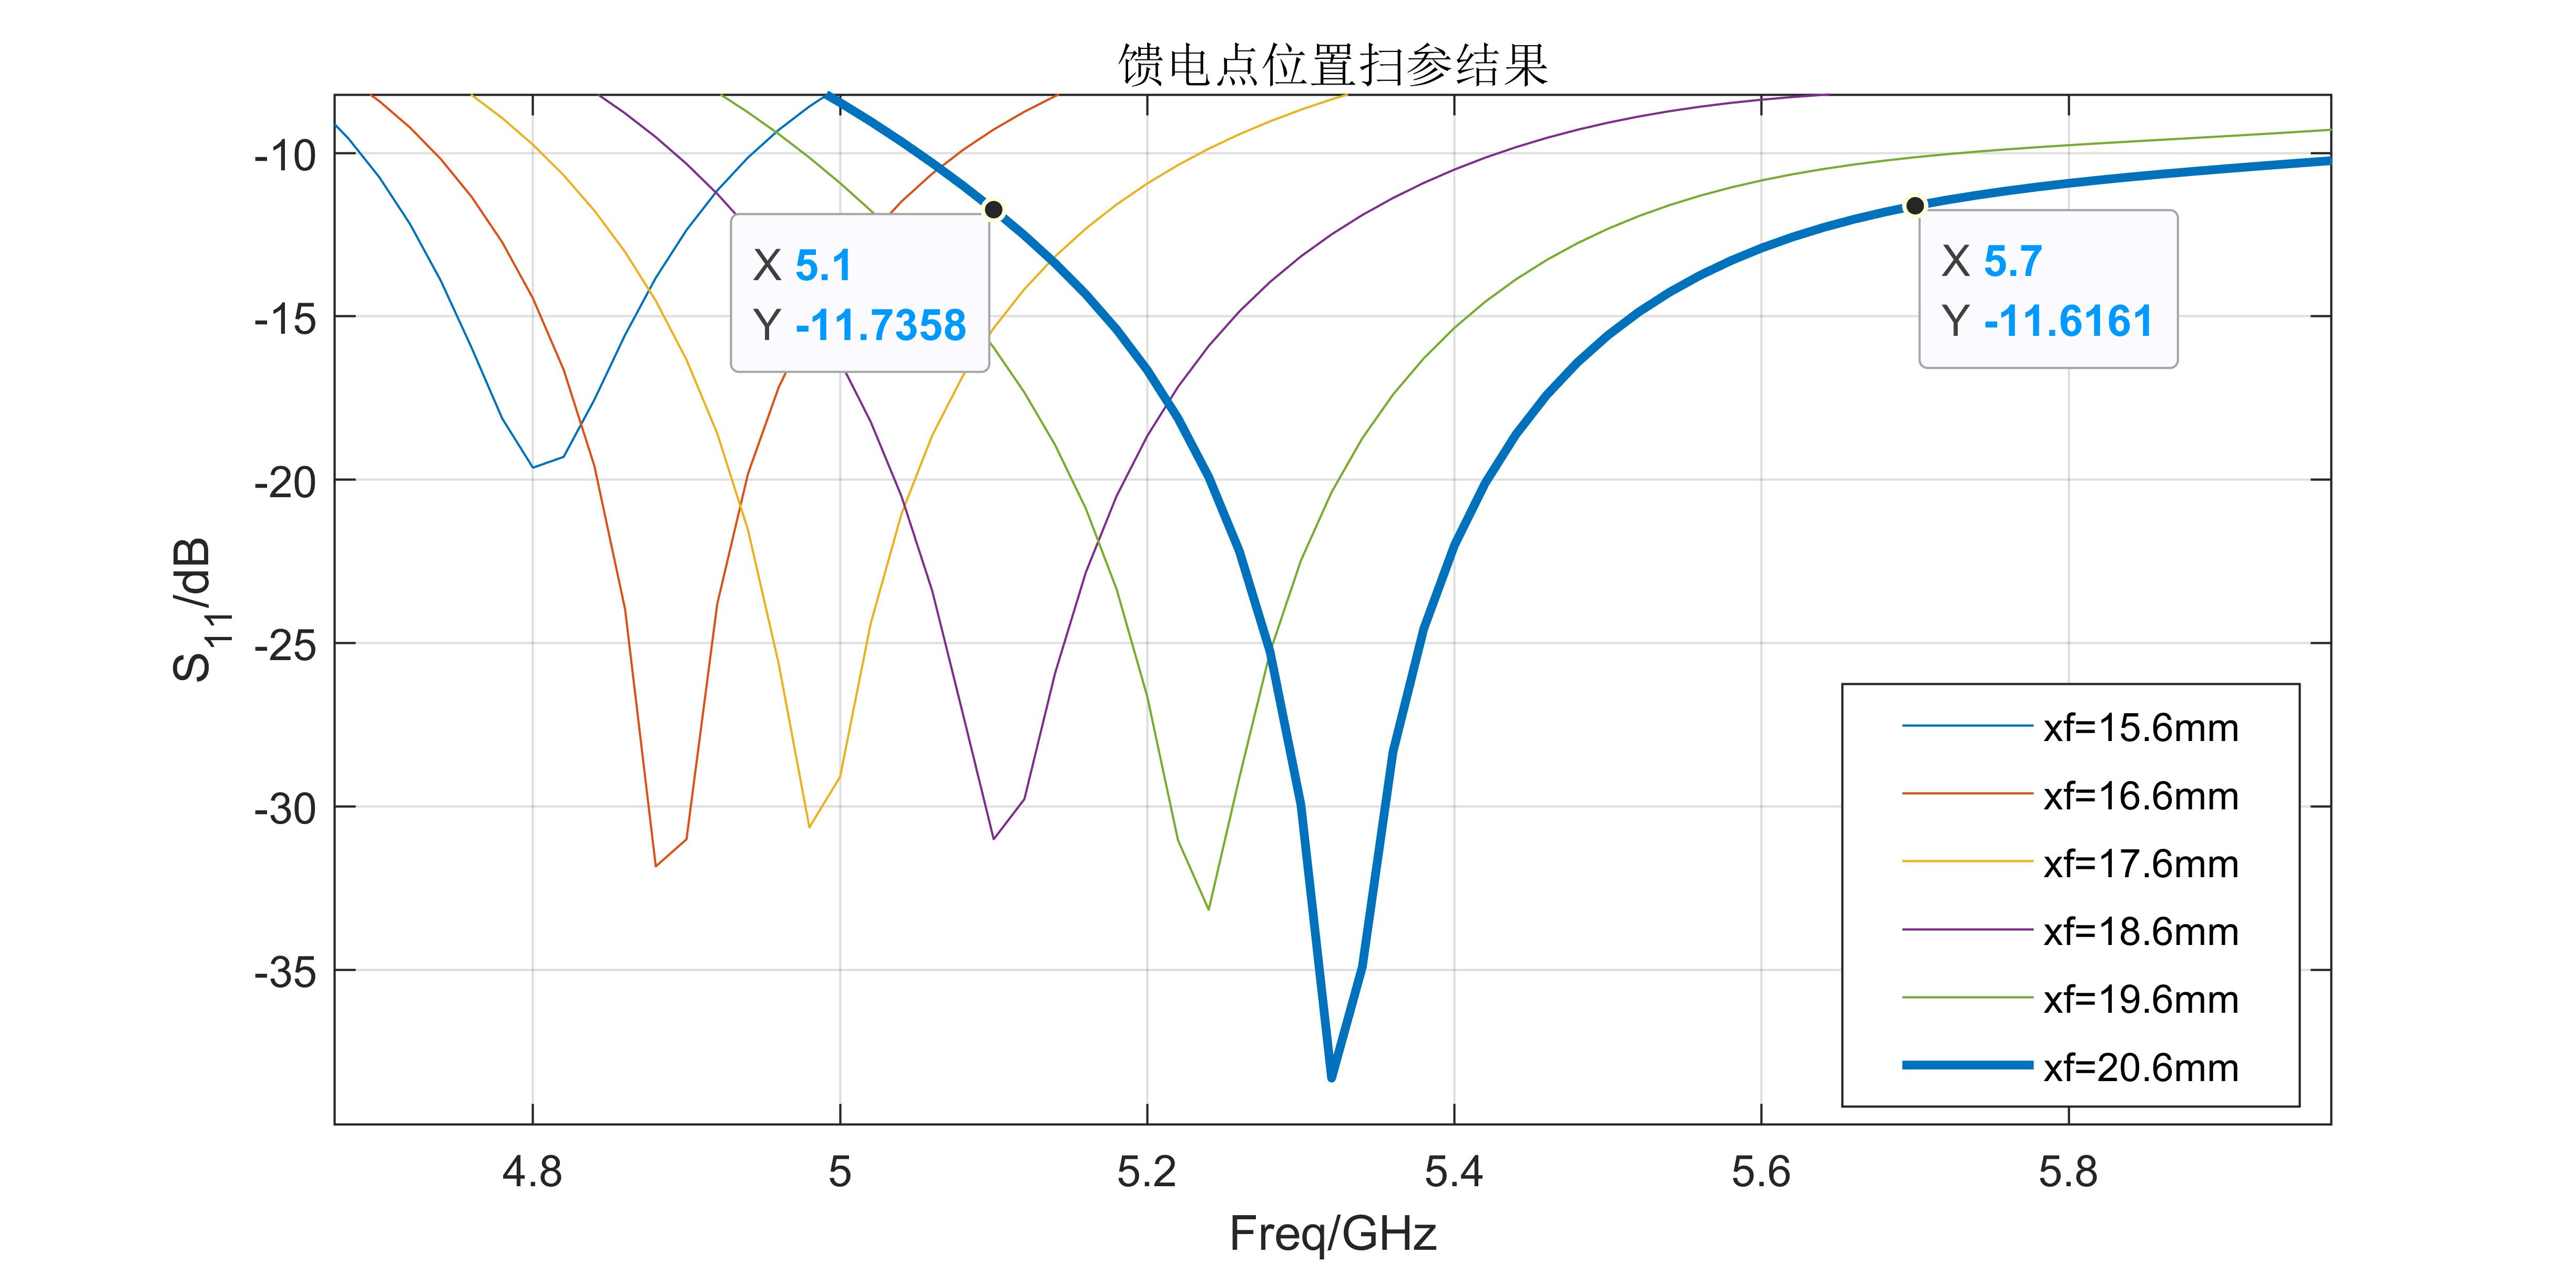
\includegraphics[height=5cm]{figs/feed_p2.jpg}
		%\caption{微带天线HFSS模型}
	\end{figure}
\end{frame}


\begin{frame}{建模仿真——{\normalsize 馈电探针半径的扫描}}
	\qquad 在保持短路导线的半径=0.5mm,
	馈电点位置$x_f=20.6mm$,短路点位置
	(8.2mm,17.5mm)不变时,改变馈电
	探针半径,其仿真结果如下图所示:
	\begin{figure}[htbp]
		\centering
		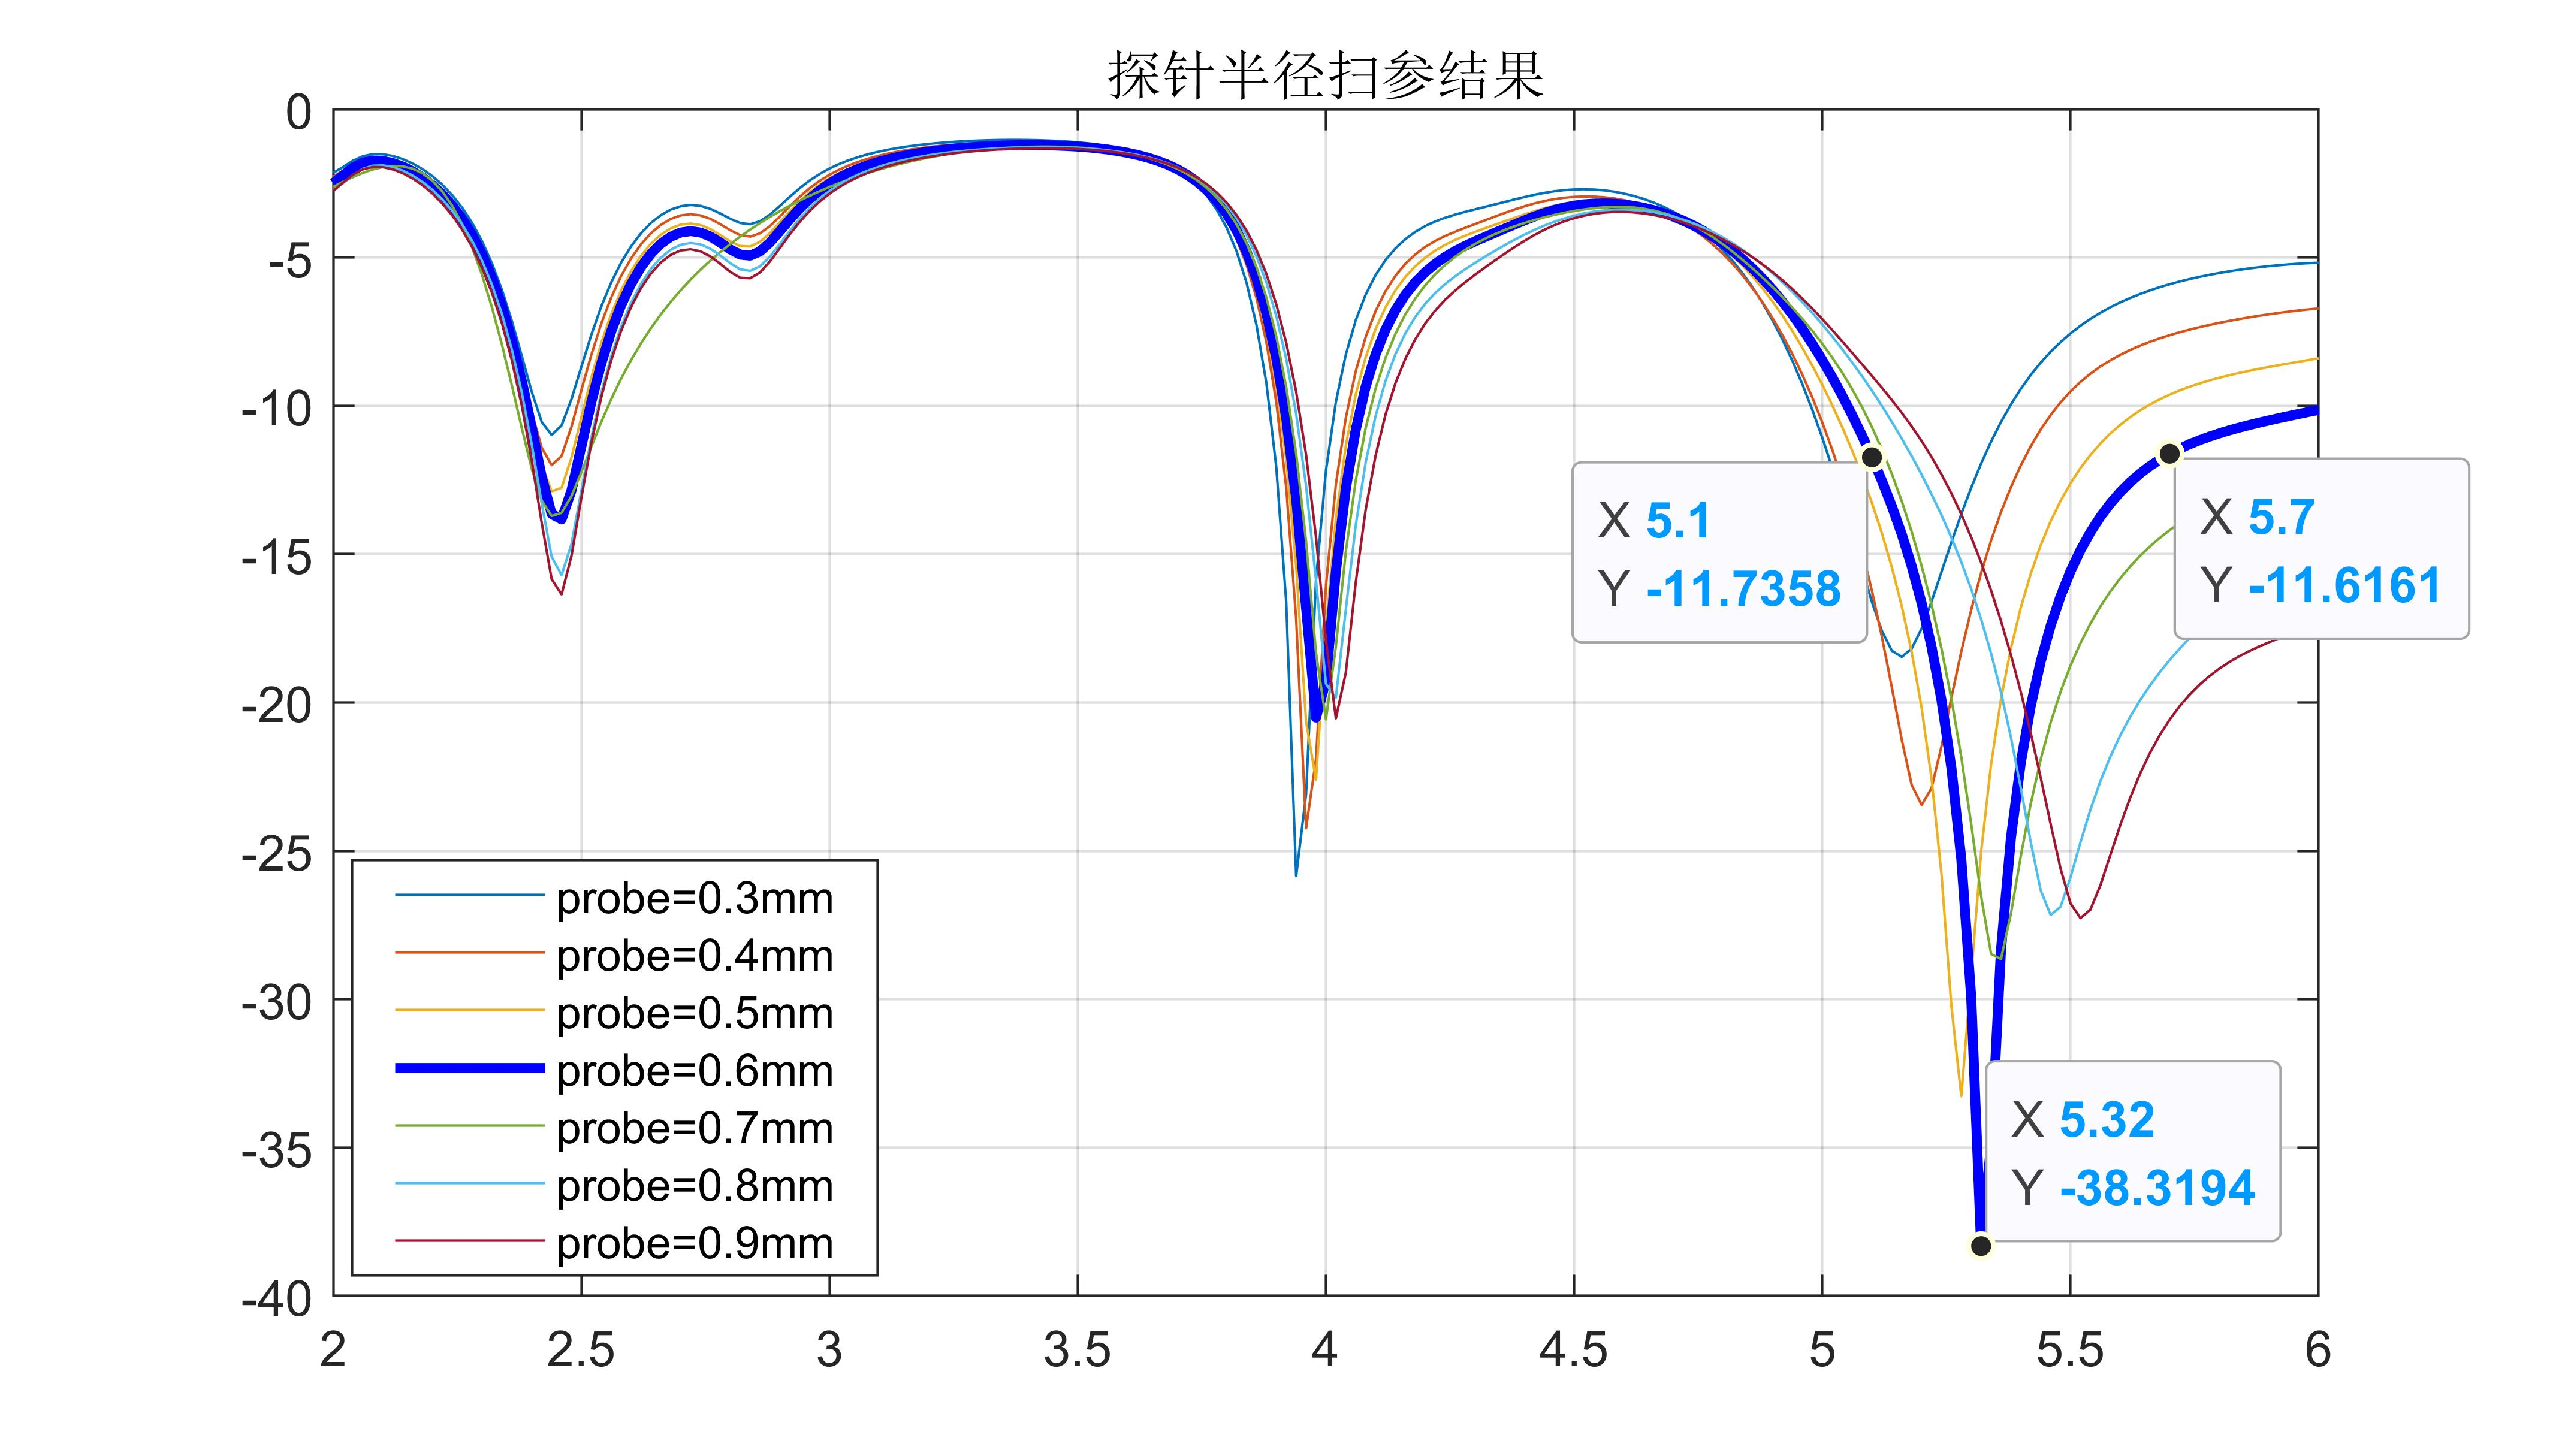
\includegraphics[height=5cm]{figs/probe1.jpg}
		%\caption{微带天线HFSS模型}
	\end{figure}
\end{frame}

\begin{frame}{建模仿真——{\normalsize 馈电探针半径的扫描}}
	\qquad 根据仿真结果我们可以知道,
	随着馈电探针的半径增大,
	其高频段谐振点频率右移,低
	频段的$S_{11}$参数变得更优。在探针半径为0.6mm时,5.1GHz和5.5GHz时
	$S_{11}$分别为-11.73dB和-15.58dB,满足要求且最佳。
	\begin{figure}[htbp]
		\centering
		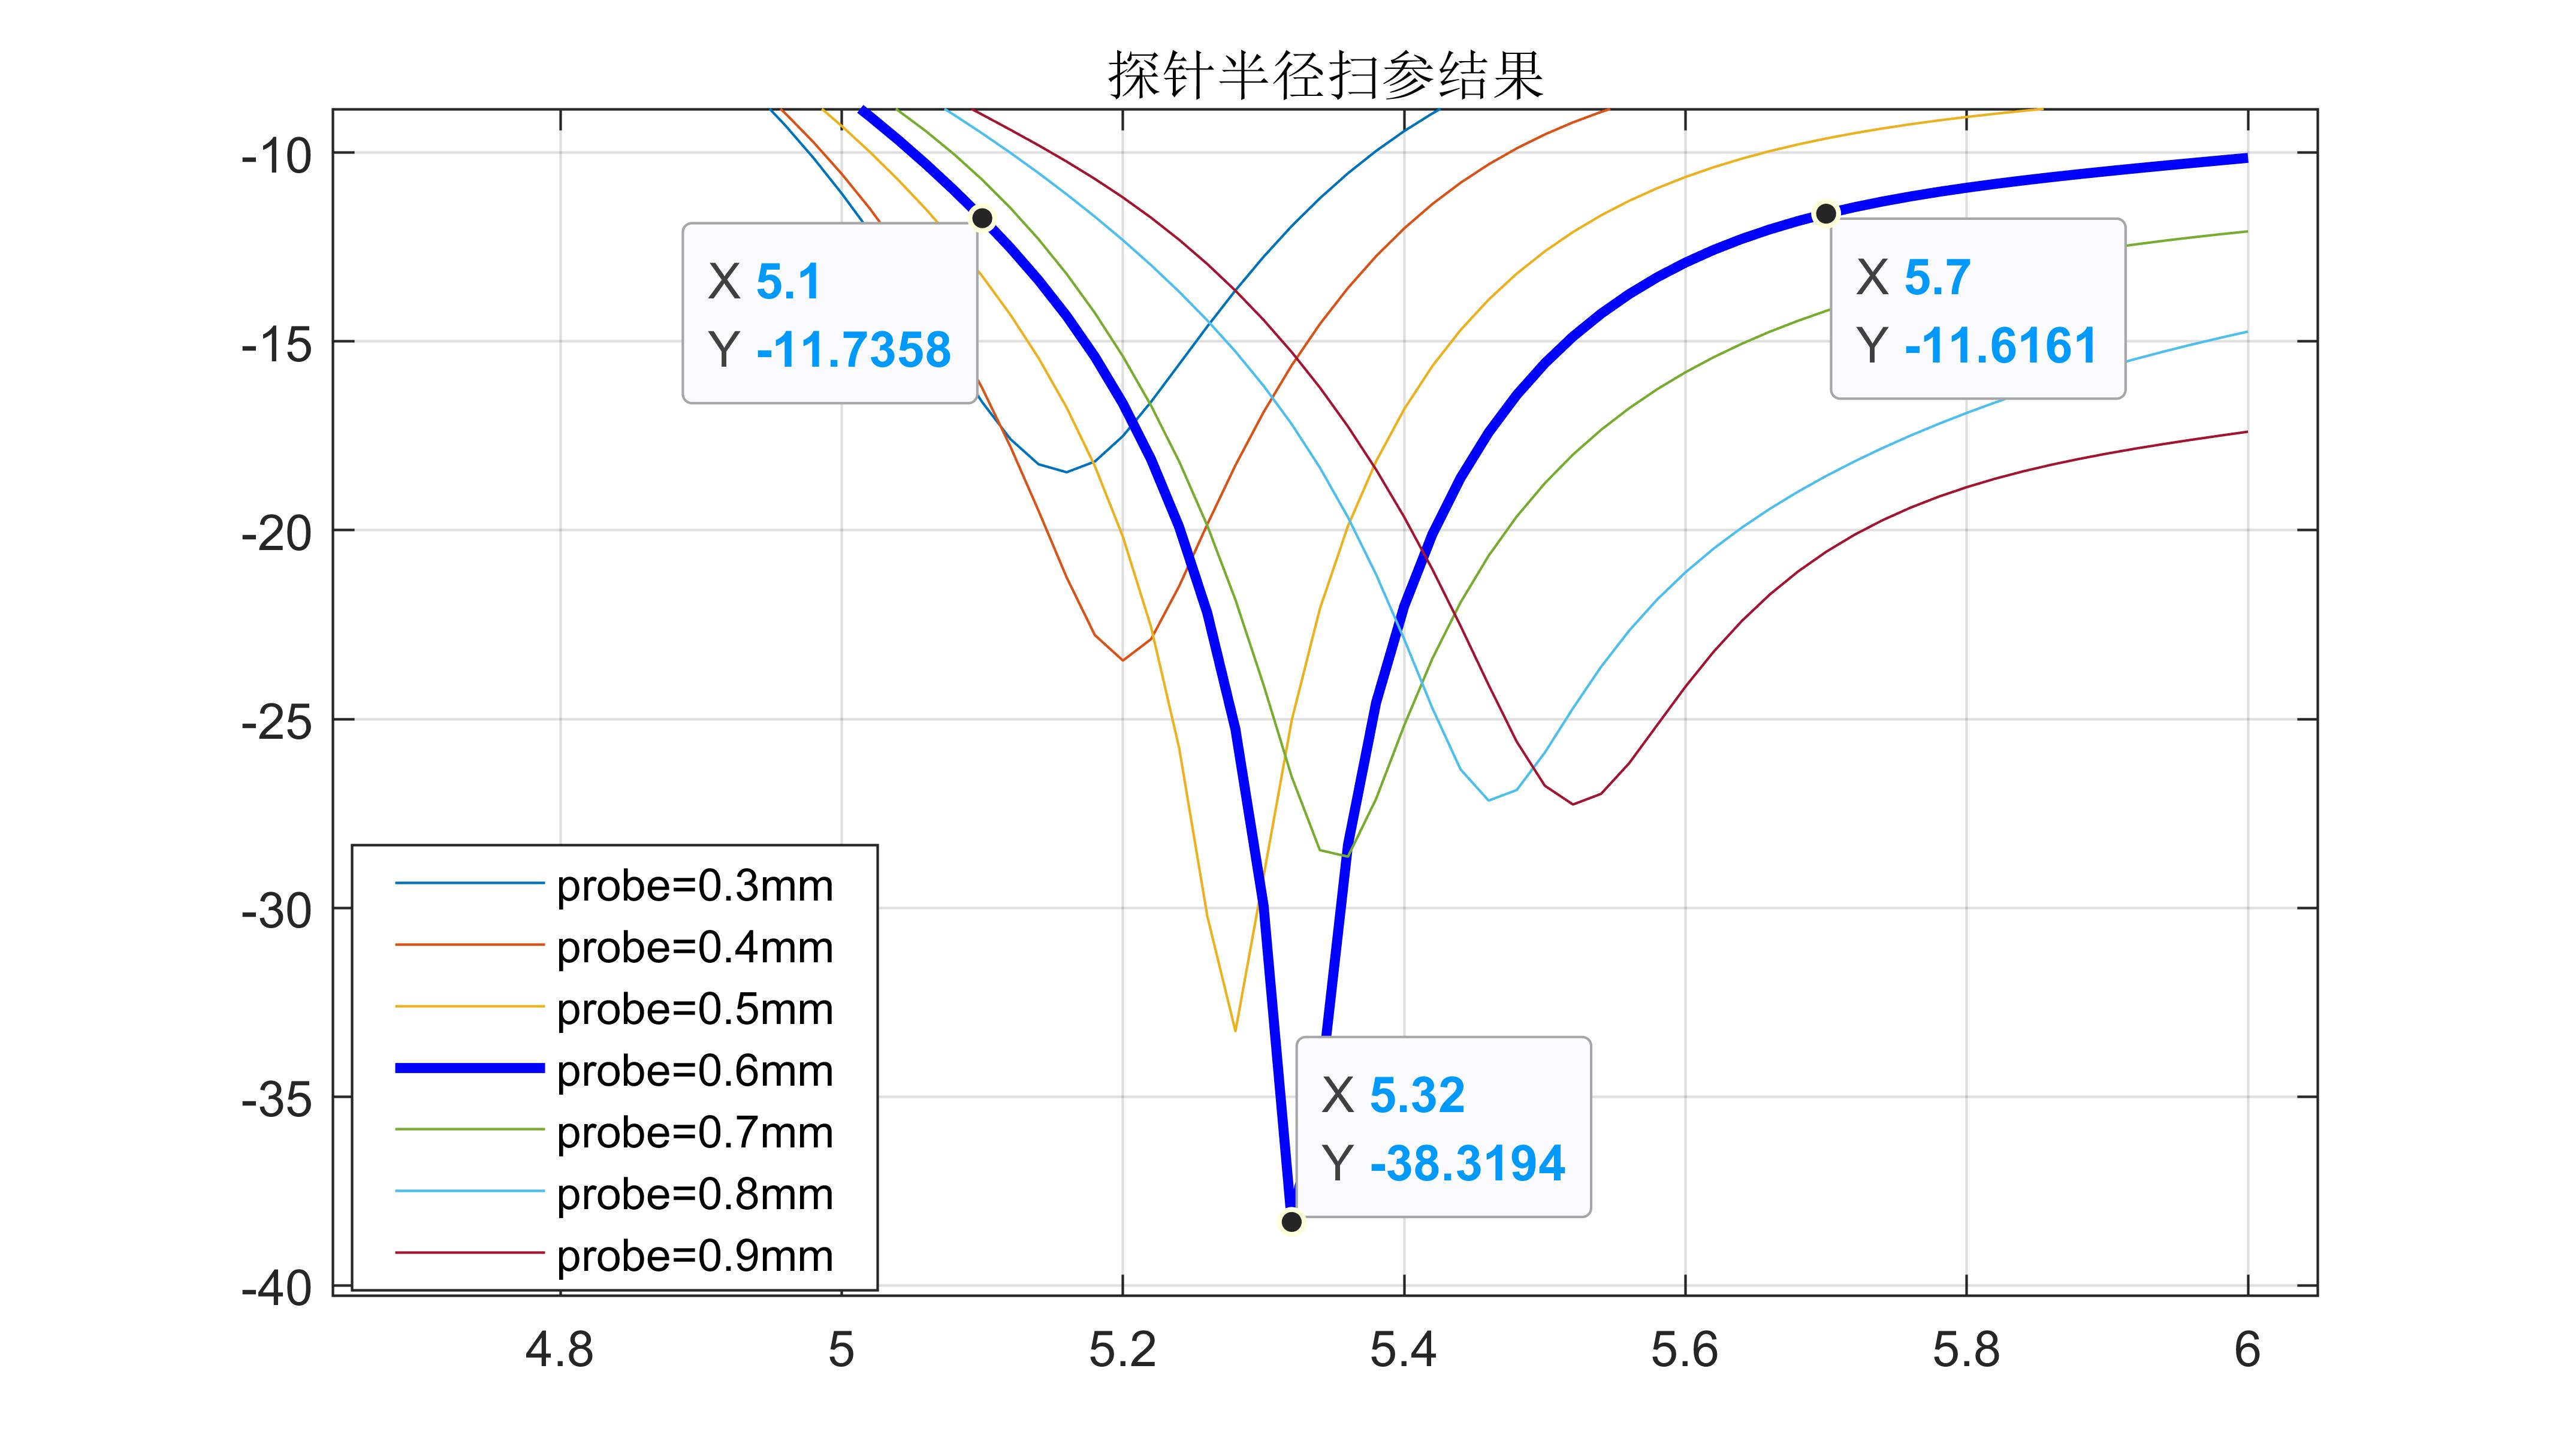
\includegraphics[height=5cm]{figs/probe2.jpg}
		%\caption{微带天线HFSS模型}
	\end{figure}
\end{frame}

\begin{frame}{建模仿真——{\normalsize 通过仿真所确定的参数}}
	\begin{table}
	\begin{tabular}{|p{6cm}|p{3cm}|}
		\hline
		参数名称& 值(mm)\\
		\hline 
		
		\hline
		短路点纵轴坐标$y_d$& 17.5\\
		\hline
		短路导线半径		& 0.5\\
		\hline
		馈电点横轴坐标$x_f$& 20.6\\
		\hline
		馈电探针半径&0.6\\
\hline
	\end{tabular}	
	\end{table}
\end{frame}
\begin{frame}{建模仿真——{\normalsize 参数确定后的结果图}}
	\qquad 在参数确定后画出其$S_{11}$图,结果如下。可看到各项指标均满足设计要求。
	\begin{figure}[htbp]
		\centering
		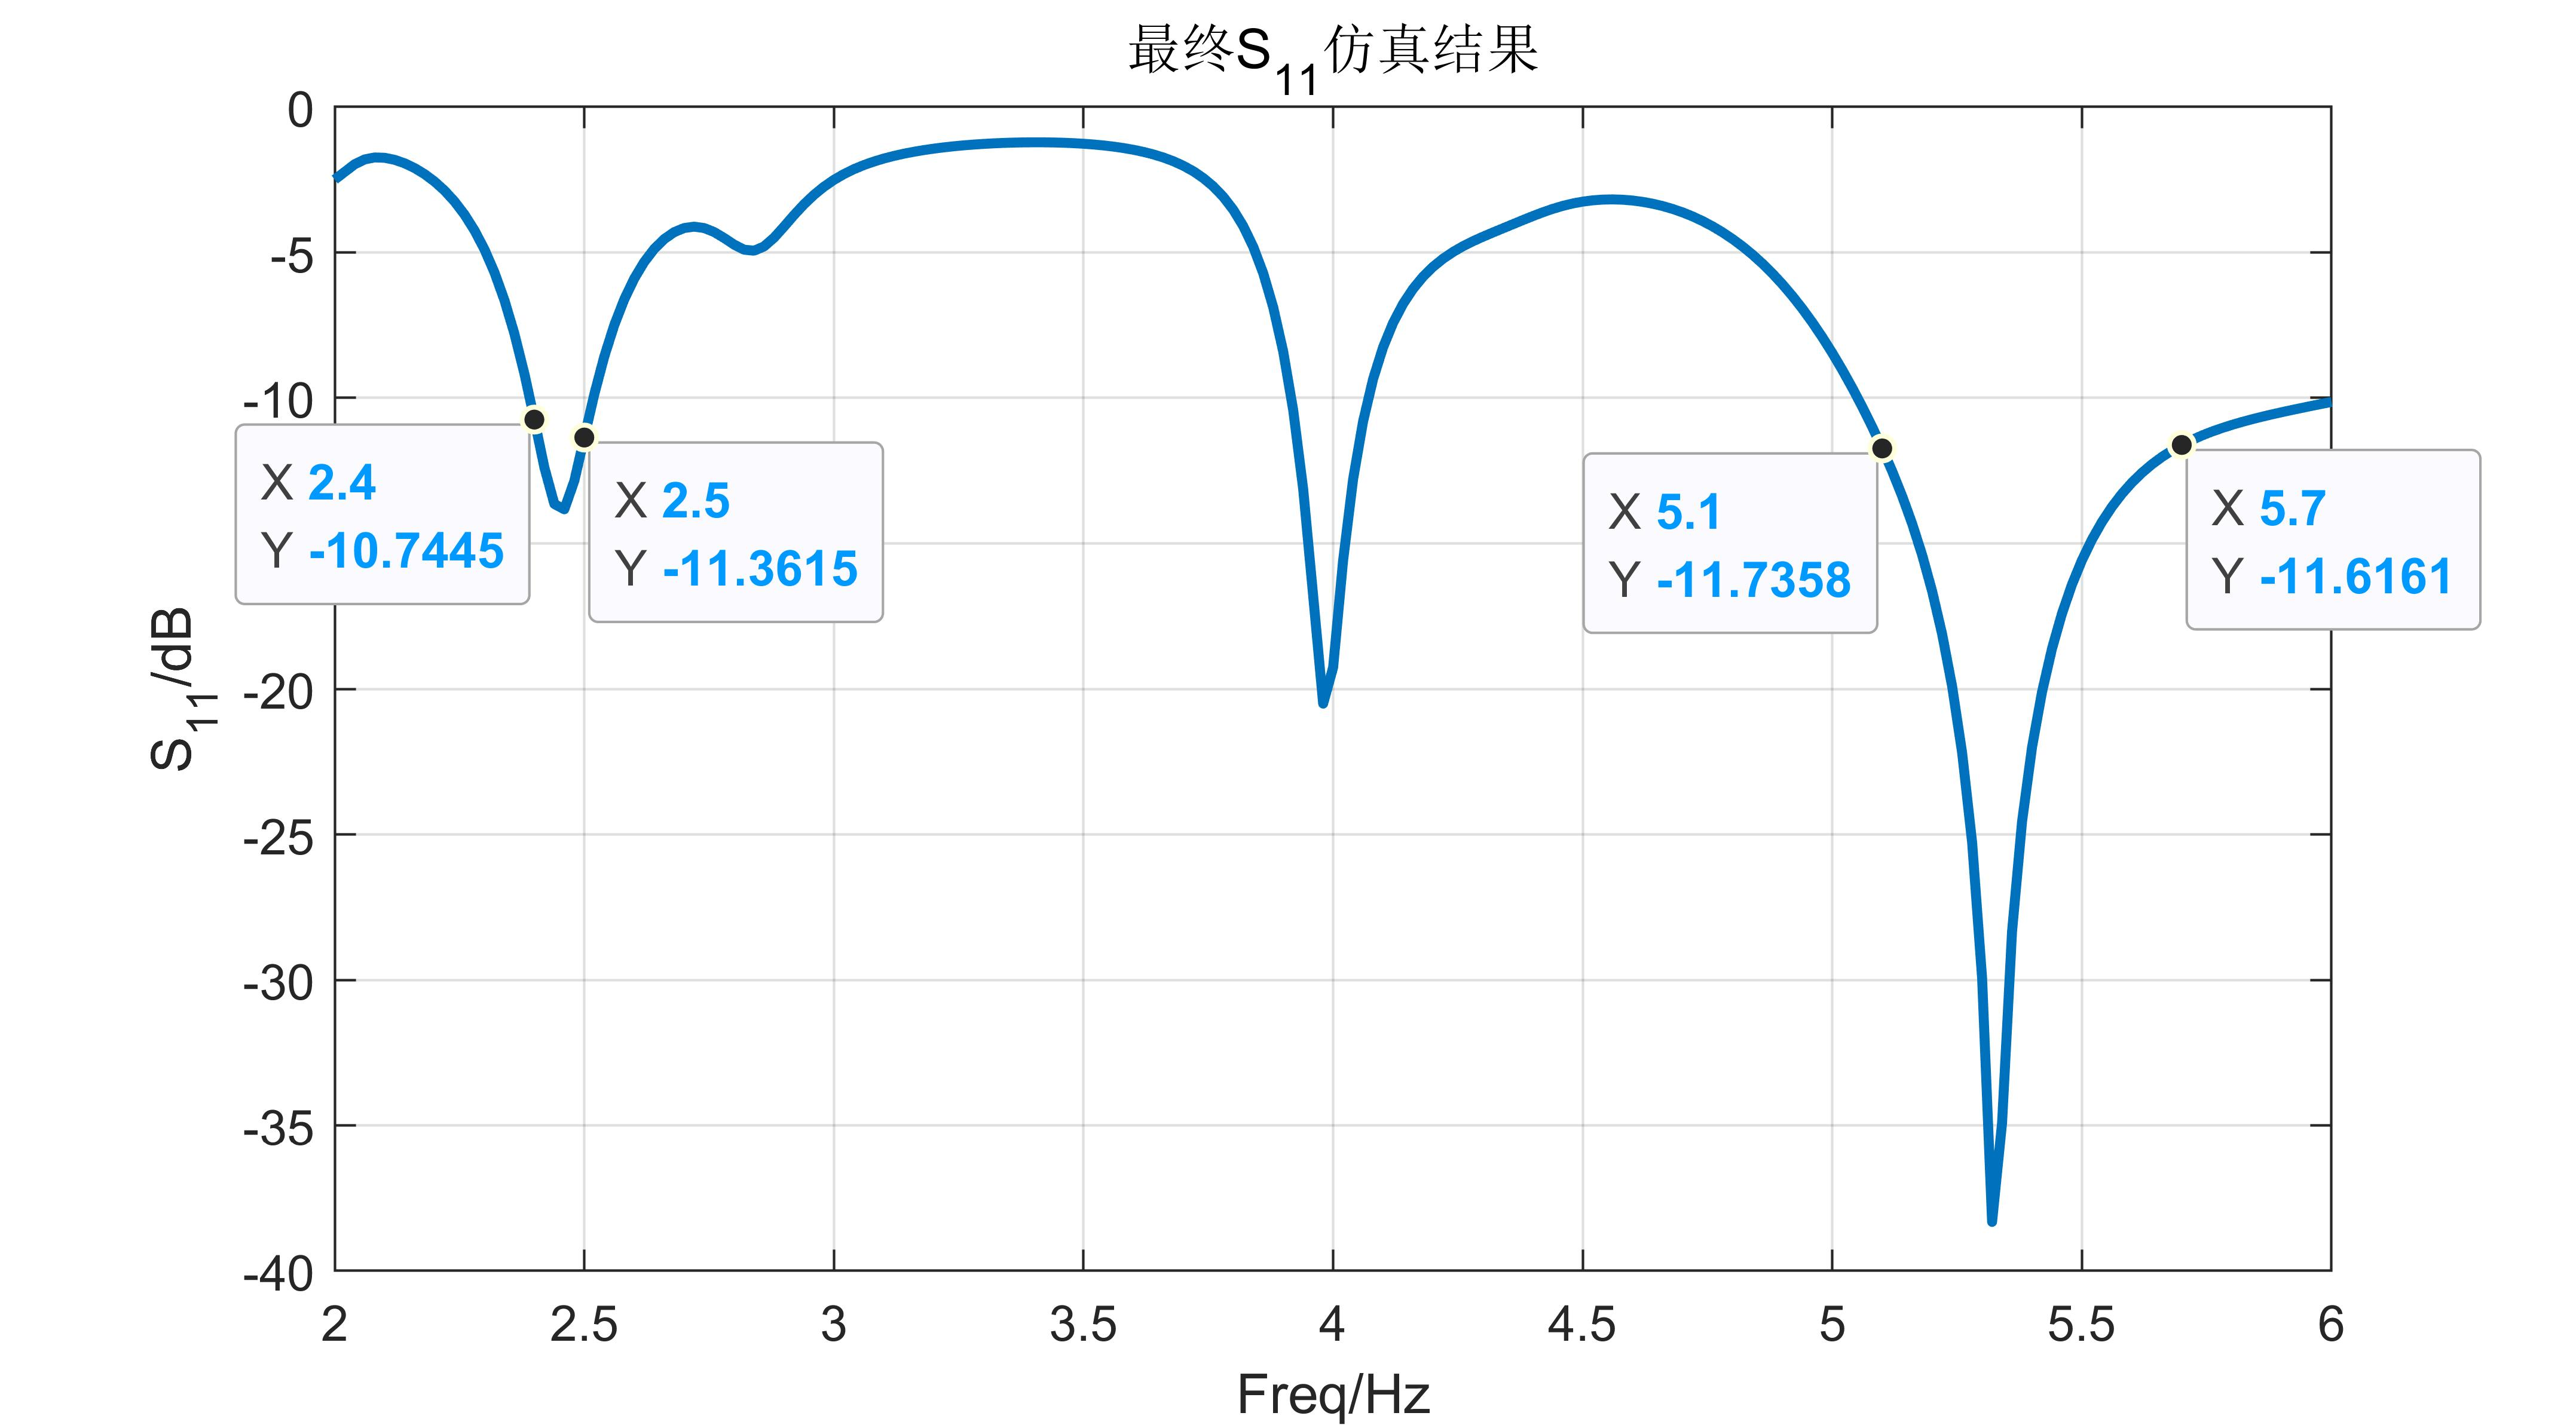
\includegraphics[height=5cm]{figs/final_S11.jpg}
		%\caption{微带天线HFSS模型}
	\end{figure}
\end{frame}

\begin{frame}{建模仿真——{\normalsize 天线增益方向图}}
	\qquad 在参数确定后画出其增益方向图如下。天线在2.45GHz的增益为6.35dB,满足要求。
	\begin{figure}[htbp]
		\centering
		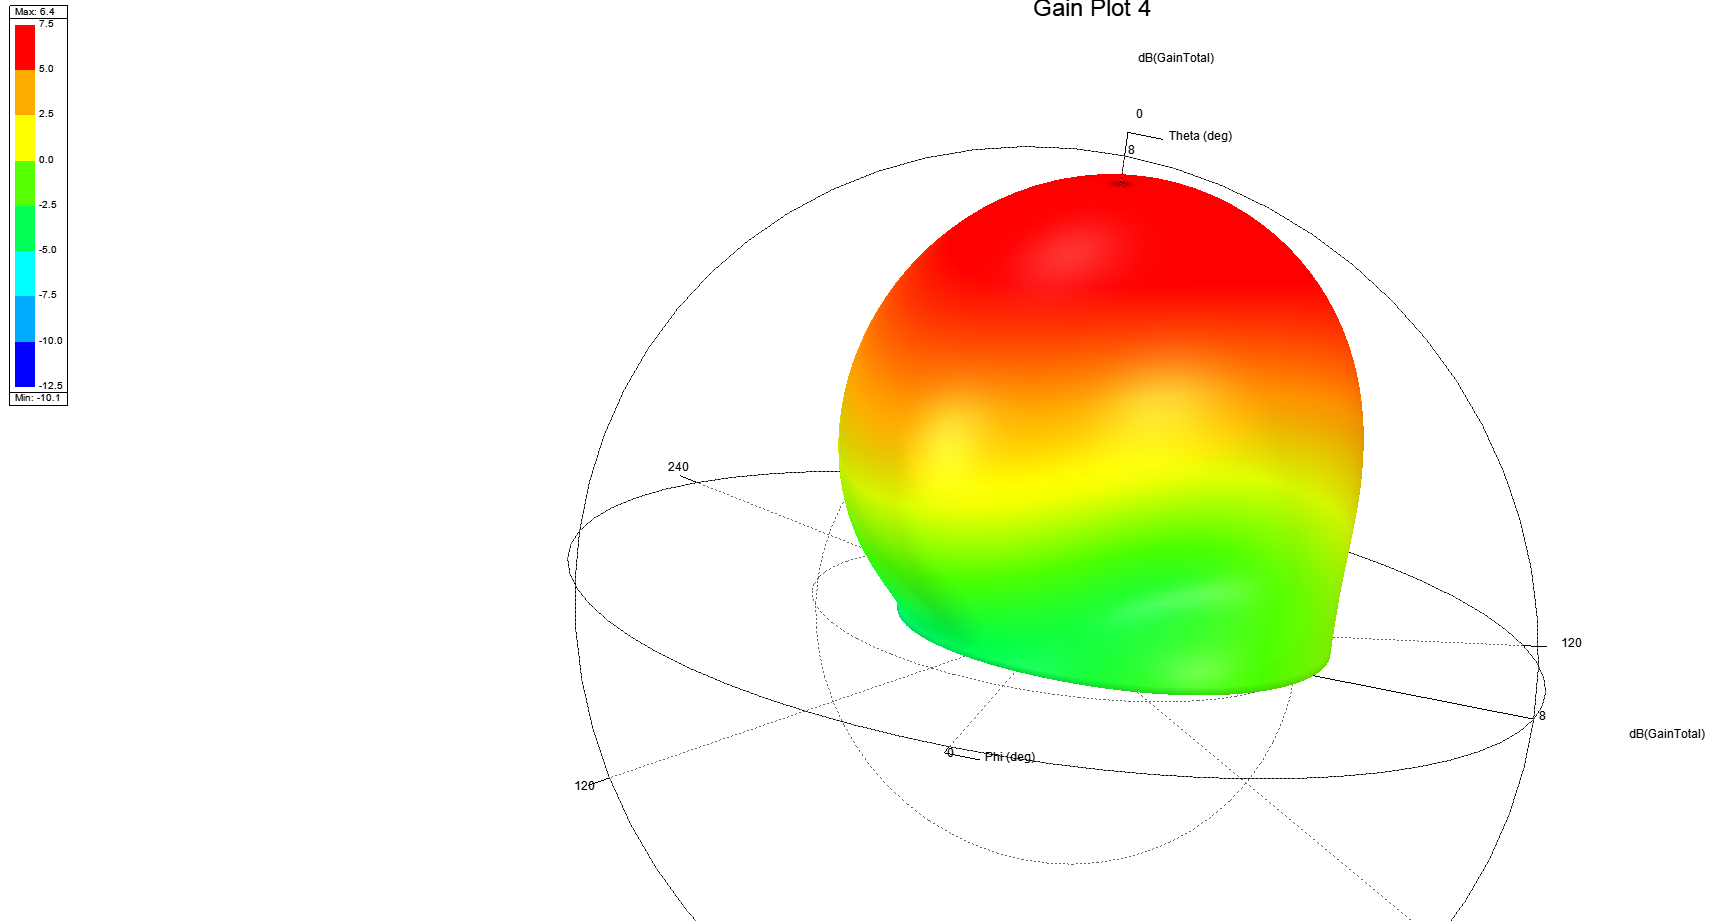
\includegraphics[height=5cm]{figs/15.png}
		%\caption{微带天线HFSS模型}
	\end{figure}
\end{frame}

\begin{frame}{建模仿真——{\normalsize 天线增益方向图}}
	\qquad 在参数确定后画出其增益方向图如下。天线在5.5GHz的增益为9.63dB,满足要求。
	\begin{figure}[htbp]
		\centering
		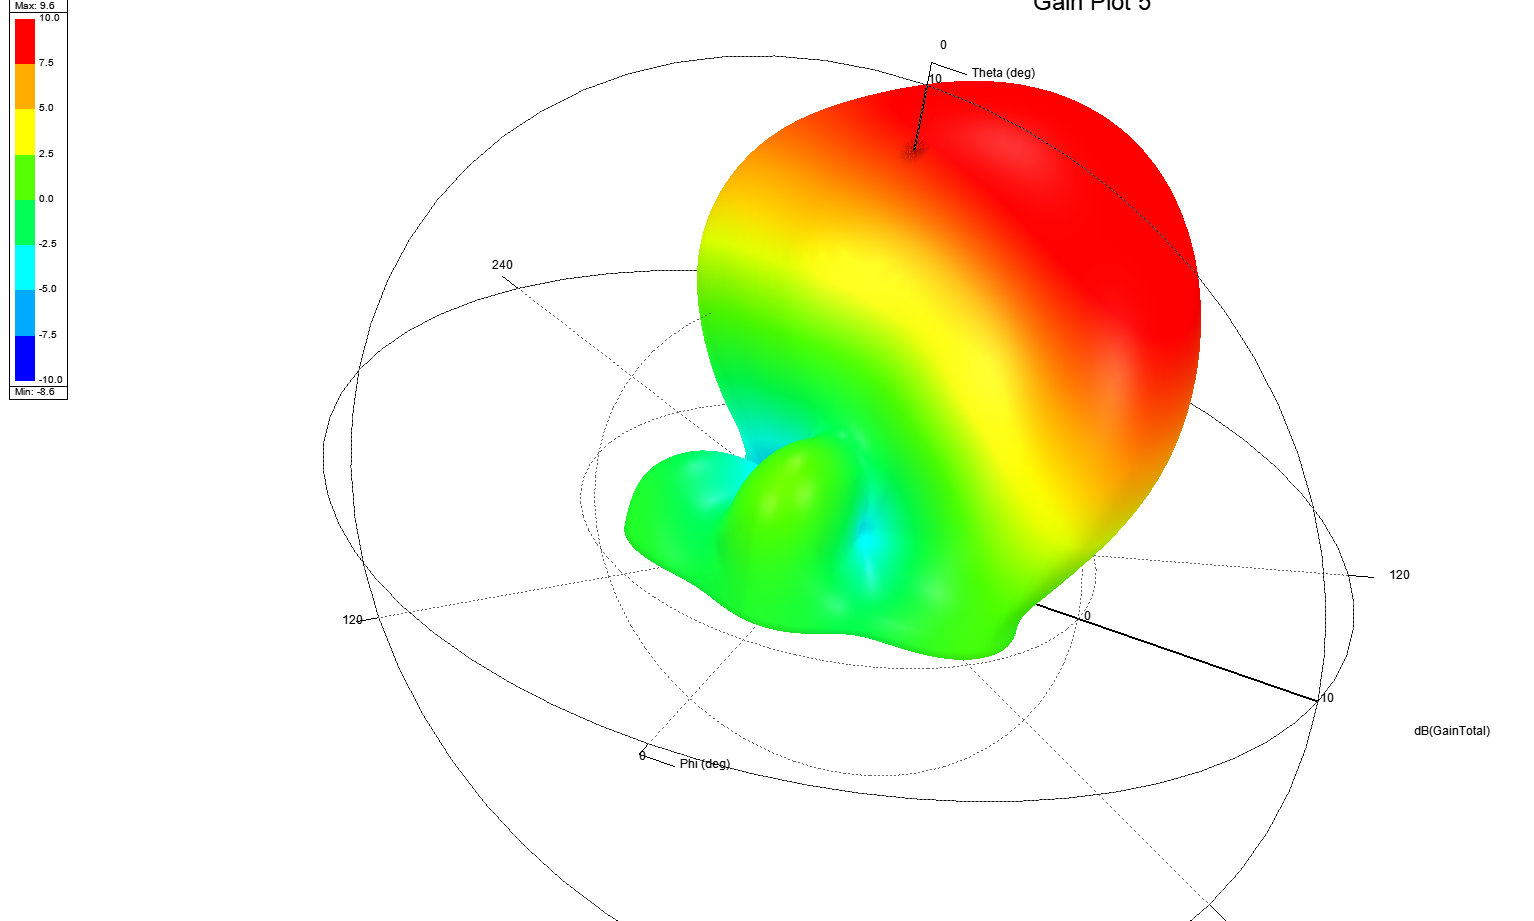
\includegraphics[height=5cm]{figs/14.png}
		%\caption{微带天线HFSS模型}
	\end{figure}
\end{frame}


\section{实物加工及测试}
\begin{frame}{实物加工及测试——{\normalsize 实物图}}
	\qquad 在通过仿真确定好天线的各项参数后,
	便进行实物加工,并测试。实物图片如图(\ref{1})、
	图(\ref{2})所示。
	\begin{figure}[htbp]
		\centering
		\includegraphics[height=5cm]{figs/1_1.png}
		\caption{天线正面图}
		\label{1}
	\end{figure}
\end{frame}

\begin{frame}{实物加工及测试——{\normalsize 实物图}}
	\begin{figure}[htbp]
		\centering
		\includegraphics[height=6cm]{figs/2a.png}
		\caption{天线反面图}
		\label{2}
	\end{figure}
\end{frame}

\begin{frame}{实物加工及测试——{\normalsize $S_{11}$测试结果}}
	\qquad 运用矢量分析仪对测量天线的$S_{11}$,得到结果如下
	\begin{figure}[htbp]
		\centering
		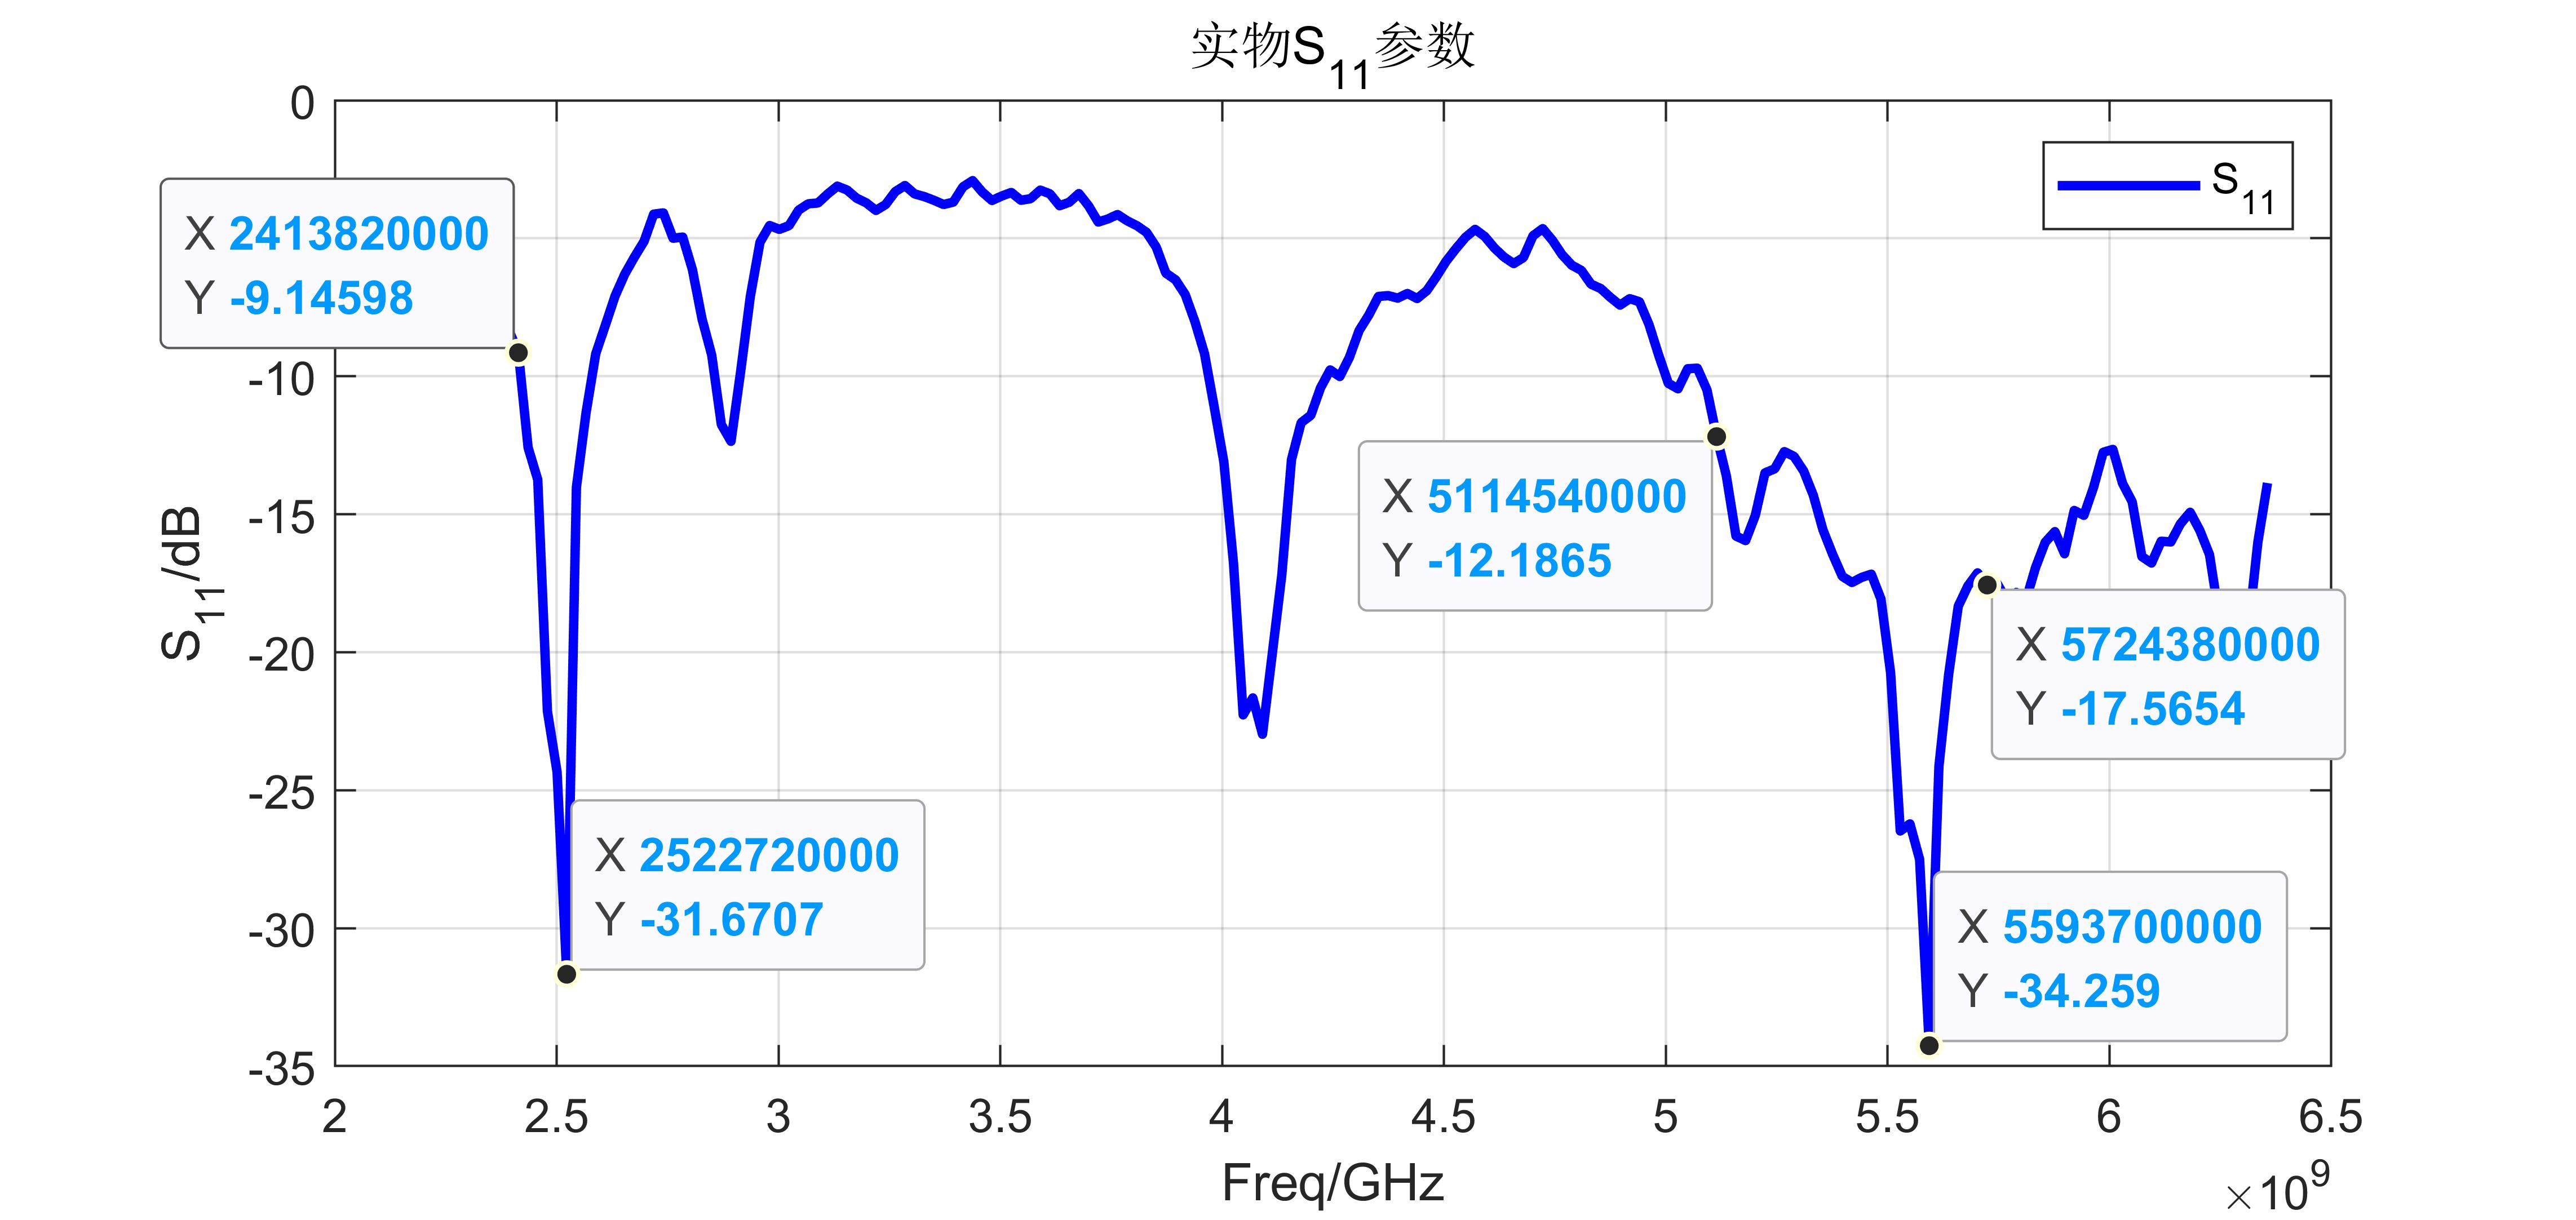
\includegraphics[height=5cm]{figs/25.jpg}
		\caption{$S_{11}$实物测试结果}
	\end{figure}
\end{frame}


\begin{frame}{实物加工及测试——{\normalsize $S_{11}$测试结果分析}}
	\qquad 运用矢量分析仪对测量天线的$S_{11}$,高频段得到结果如下。
	可以看到其$S_{11}$满足指标设计要求,且优于仿真结果。
	\begin{figure}[htbp]
		\centering
		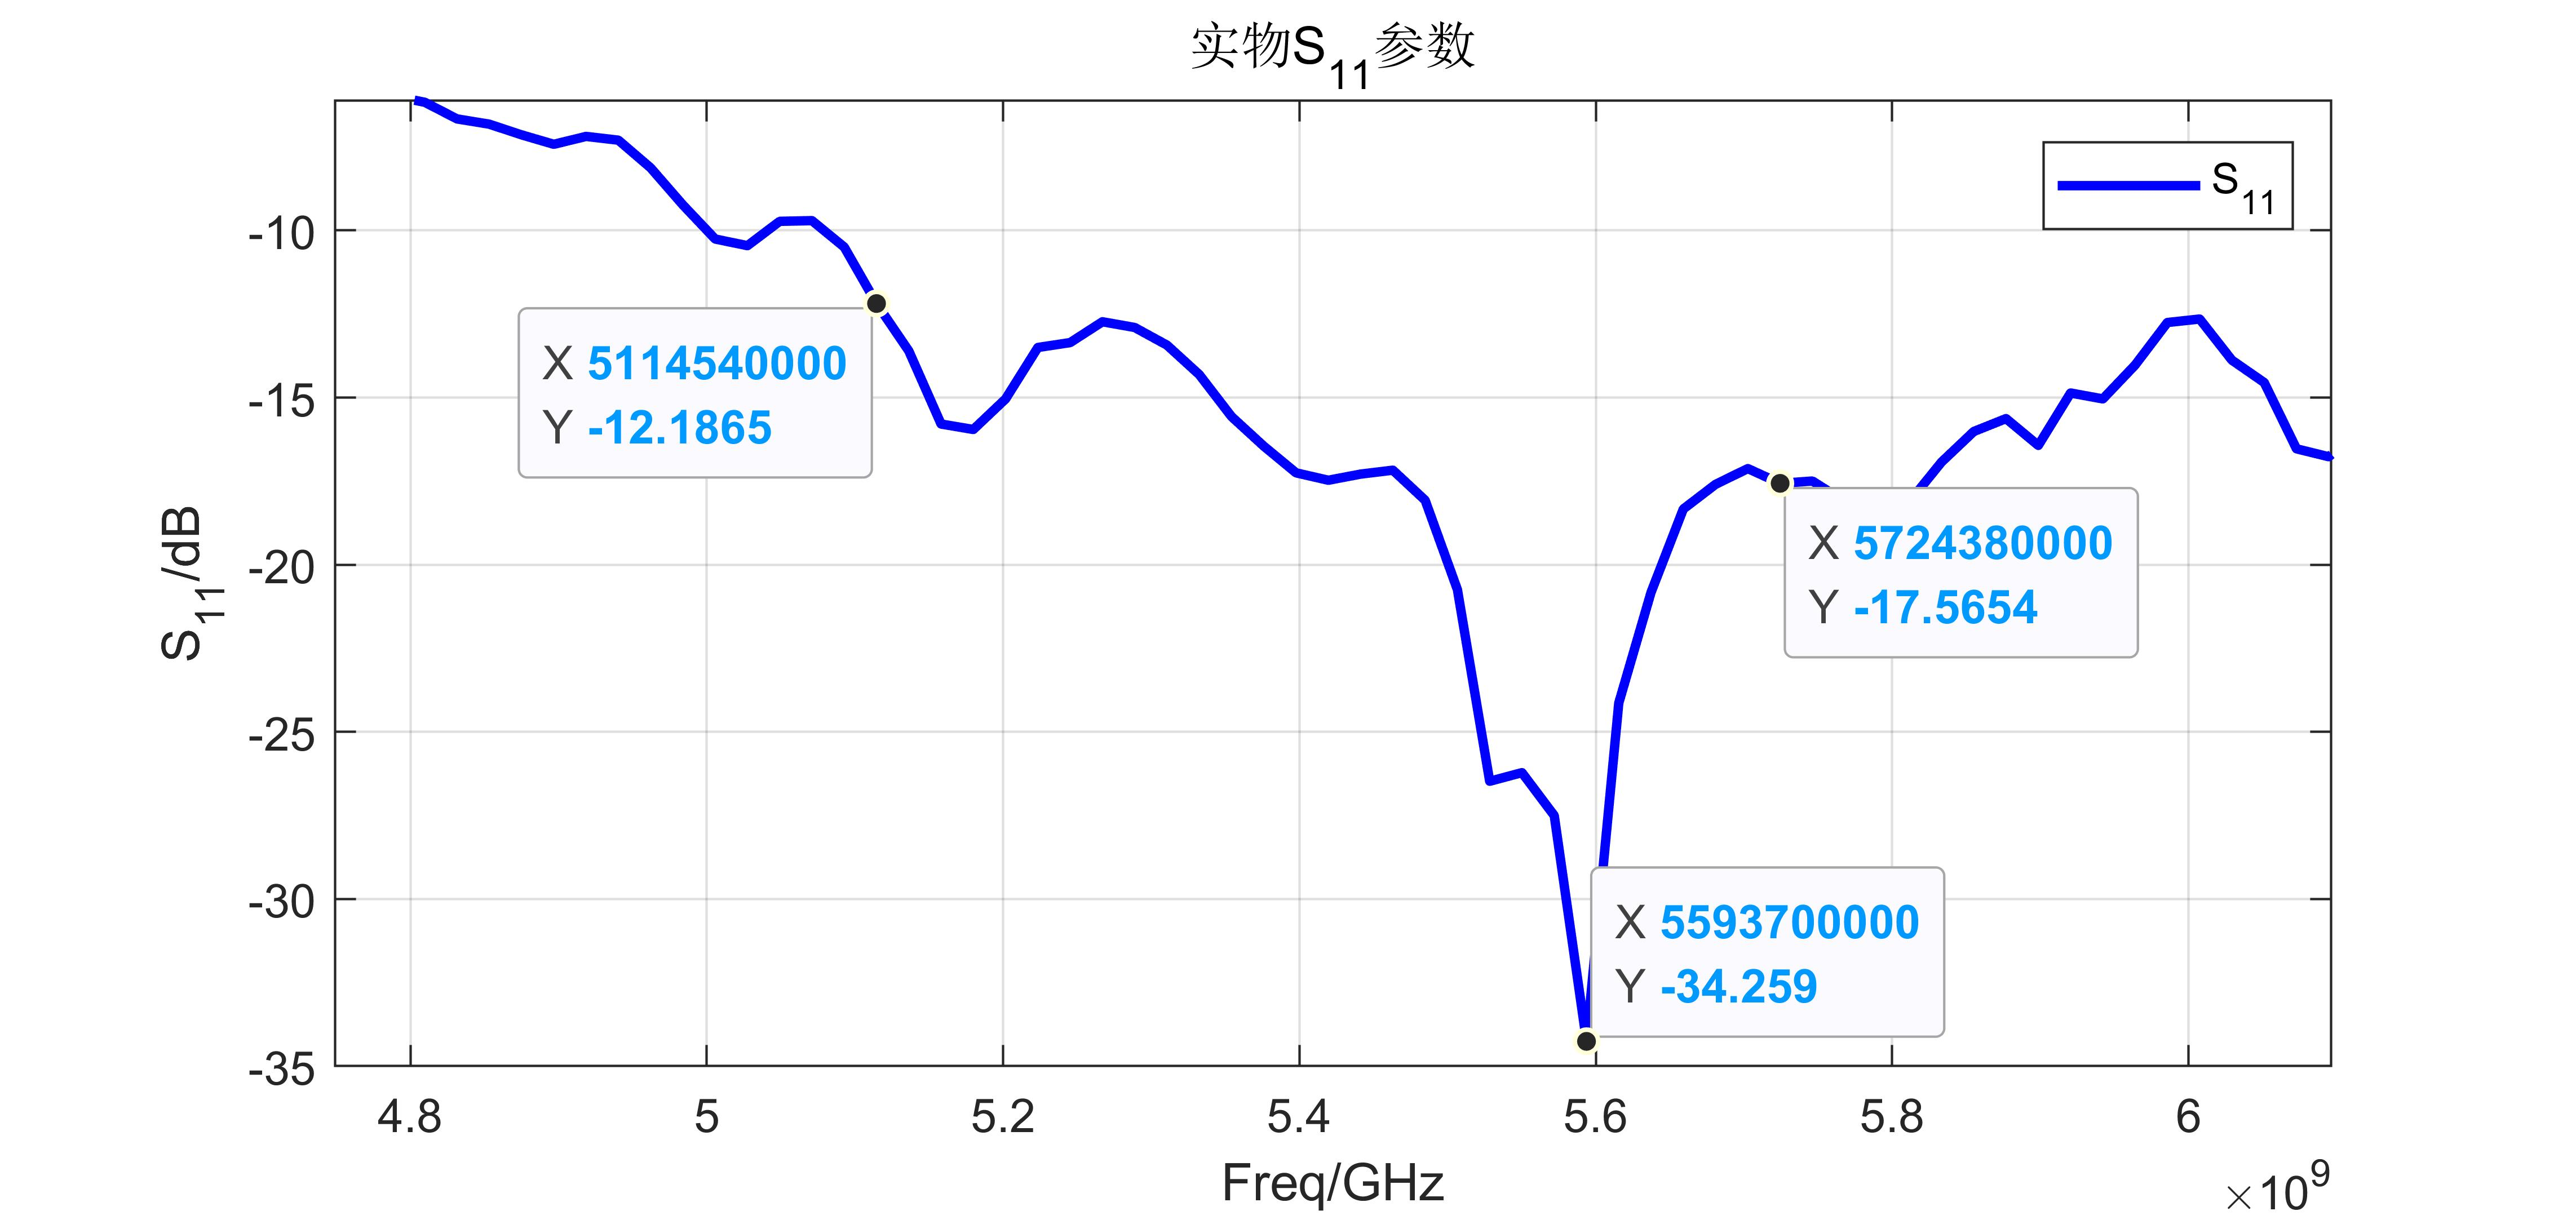
\includegraphics[height=4cm]{figs/27.jpg}
		\caption{$S_{11}$高频段测试结果}
	\end{figure}
\end{frame}

\begin{frame}{实物加工及测试——{\normalsize $S_{11}$测试结果分析}}
	\qquad 运用矢量网络分析仪对测量天线的$S_{11}$,低频段得到结果如下。
	可以看到在2.4GHz其$S_{11}$为-9.1dB左右,在2.5GHz其$S_{11}$为-31.6dB
	左右,基本满足要求。

	\begin{figure}[htbp]
		\centering
		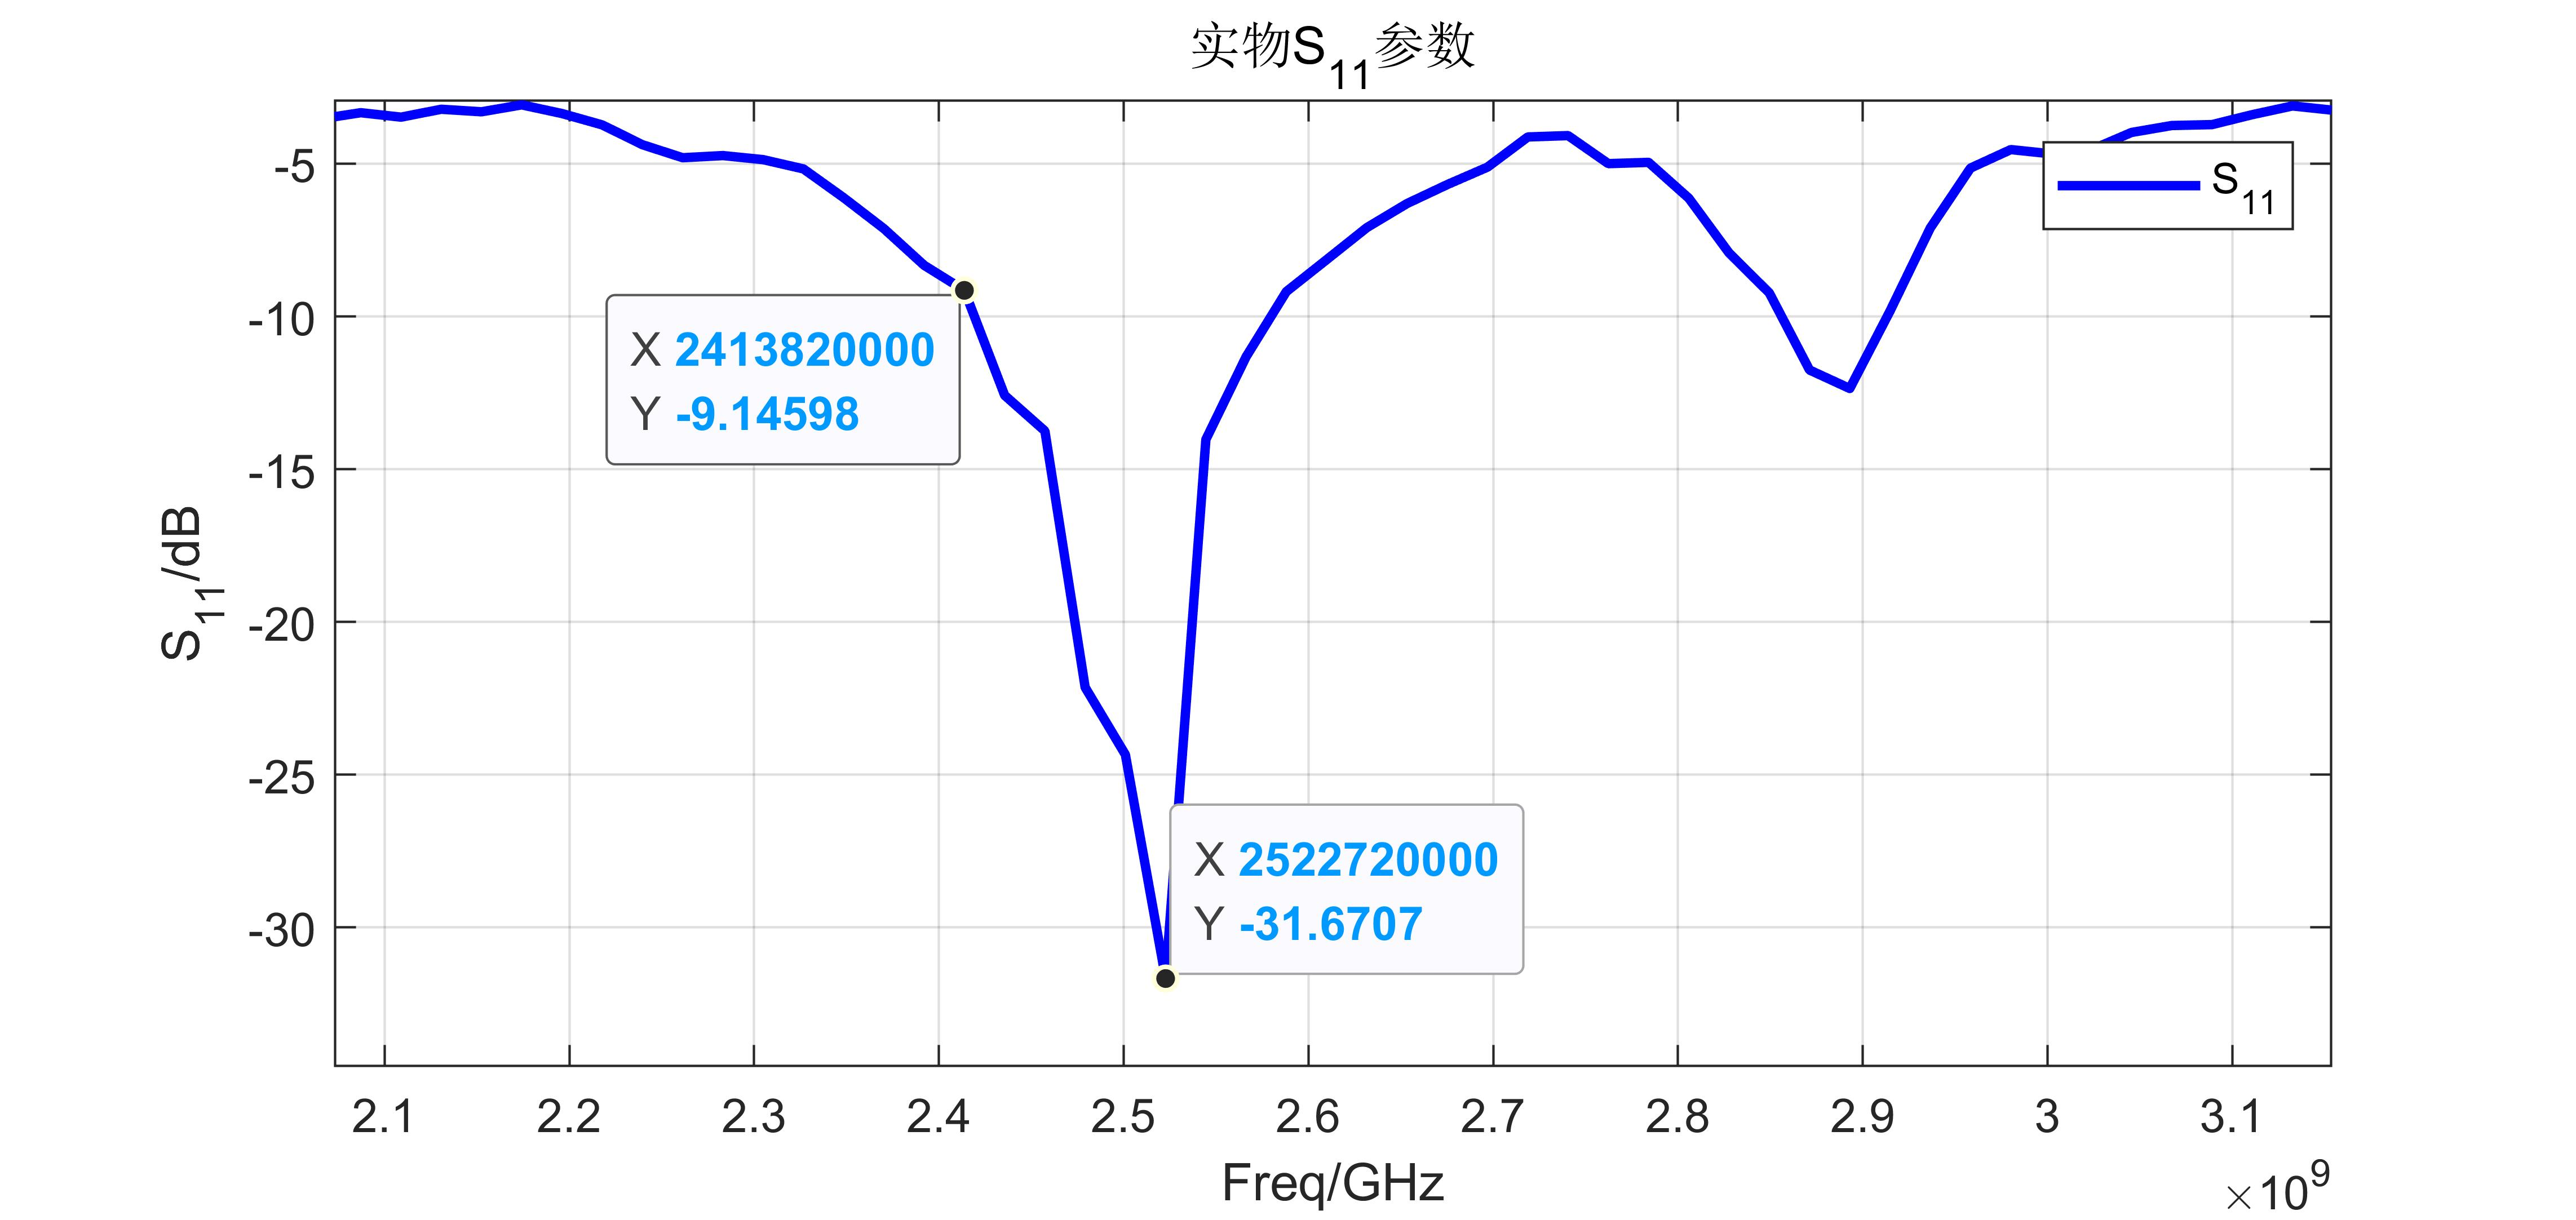
\includegraphics[height=4cm]{figs/26.jpg}
		\caption{$S_{11}$低频段测试结果}
	\end{figure}
\end{frame}

\begin{frame}{实物加工及测试——{\normalsize $S_{11}$测试仿真结果对比}}
	\qquad 
	将仿真所得的$S_{11}$和运用矢网所得的$S_{11}$进行对比,得到结果如下:

	\begin{figure}[htbp]
		\centering
		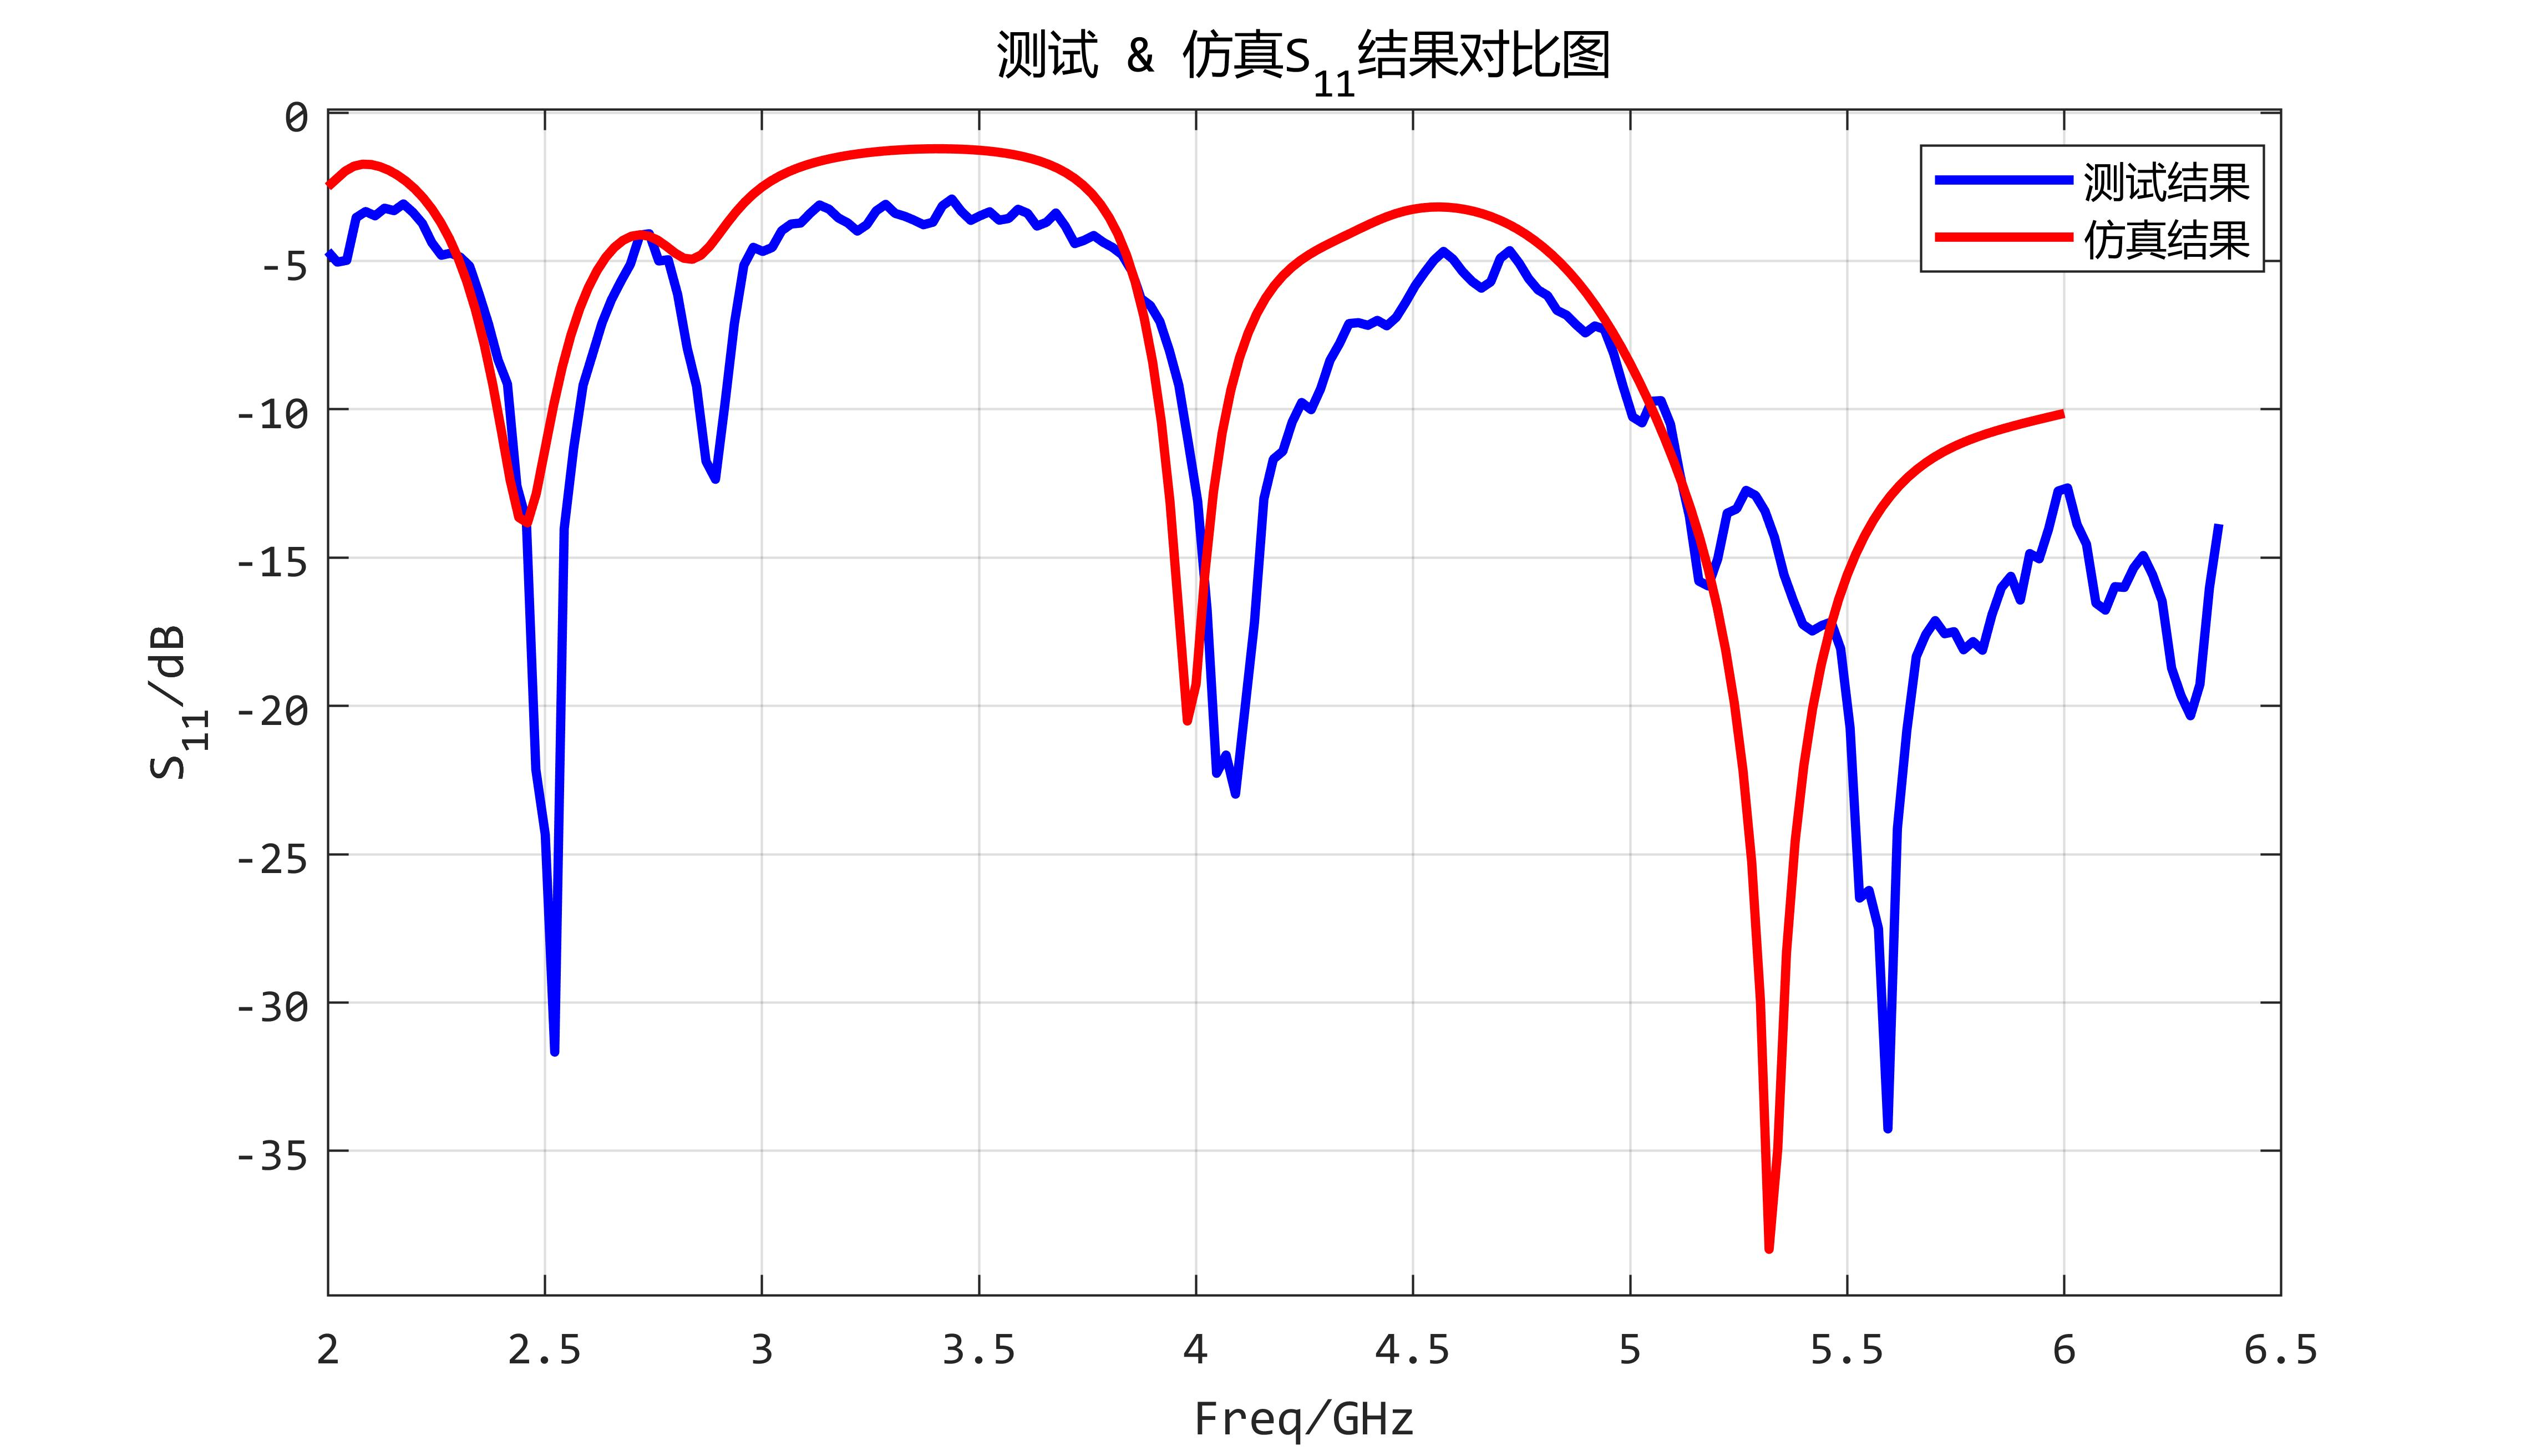
\includegraphics[height=5cm]{figs/test_simulation.jpg}
		%\caption{$S_{11}$低频段测试结果}
	\end{figure}

\end{frame}


\begin{frame}{实物加工及测试——{\normalsize $S_{11}$测试结果分析}}
	\qquad 在低频,仿真结果和测试结果有较高的吻合度;但在高频,发现
	测试结果和仿真结果有一定的偏差。\pause

	\bigskip
	\qquad 原因推断:

	\qquad 在仿真分析中,我们得到这样的结论:即影响高频的因素是馈电探针的
	位置和半径。但是在实物焊接的过程中:

	\begin{enumerate}

		\item 囿于条件限制,馈电探针的半径不能和仿真所得到的结果一致,
		相较于仿真所得的0.6mm半径较大,导致谐振点向高频移动。
		\item 由于手工焊接,导致馈电探针没有与天线垂直,而是有一定的倾斜。
		 
	\end{enumerate}
	
	
\end{frame}


\section{总结展望}

\begin{frame}{总结展望}
	\qquad 在本次项目中,我们对论文《应用于无线局域网的低剖面宽带双频微带天线的设计》进行了复现。
	\begin{enumerate}
		\item 	首先是阅读相关文献,对相关理论进行了分析和学习,并大致了解了此领域的研究状况。\pause
		\item 其次是按照论文对天线进行了建模和仿真,且在仿真中发现了一些和论文不同的数据和结果。这考验我们的批判和质疑精神。\pause
		\item 最后是对仿真模型进行了实物加工,并对实物进行了数据测试,感受并体验到了从理论到实践的过程,体会到理论和实践还是有一定距离的。因为理论只能指导实践而不能决定实践,现实中有很多不确定的因素是理论无法考虑进去的。
	\end{enumerate}
\end{frame}

\begin{frame}{总结展望}
	\qquad 本次课程设计中,我们体会到了完整的科研过程,增强了对于科研的认识,并提高了有关科研的一些基本技能。

	\qquad 希望以后能在科研的路上有所作为!
\end{frame}

\section{参考文献}
\begin{frame}{参考文献}

	[1]罗歆瑶,袁家德.应用于无线局域网的低剖面宽带双频微带天线的设计[J].福州大学学报(自然科学版),2017,45(06):829-832.

	[2]张磊,潘传红,栾秀珍,刘占友,王均松.一种用于WLAN的双短路针调谐U形槽加载的双频微带贴片天线[J].大连海事大学学报,2007(S2):147-148.

	[3]李鑫,丁军,吕晓德.一种用于WLAN的U形槽加载的双频贴片微带天线[J].中国科学院研究生院学报,2007(03):380-384.

	[4]杨晋乾,王旭光.一种应用于5G的双频微带天线设计[J].信息通信,2020(06):83-85.

	[5]杨晋乾,王旭光.一种应用于5G的双频微带天线设计[J].信息通信,2020(06):83-85.

\end{frame}

\begin{frame}
\begin{center}
	\Huge \textit{谢谢聆听!}
\end{center}
	
\end{frame}
\end{document}